%%
%% This is file `manuscript.tex',
%% generated with the docstrip utility.
%%
%% The original source files were:
%%
%% samples.dtx  (with options: `all,proceedings,manuscript')
%%
%% IMPORTANT NOTICE:
%%
%% For the copyright see the source file.
%%
%% Any modified versions of this file must be renamed
%% with new filenames distinct from manuscript.tex.
%%
%% For distribution of the original source see the terms
%% for copying and modification in the file samples.dtx.
%% (The sources need not necessarily be in the same archive or directory.)
%%
%% Commands for TeXCount
%TC:macro \cite [option:text,text]
%TC:macro \citep [option:text,text]
%TC:macro \citet [option:text,text]
%TC:envir table 0 1
%TC:envir table* 0 1
%TC:envir tabular [ignore] word
%TC:envir displaymath 0 word
%TC:envir math 0 word
%TC:envir comment 0 0
%%
\documentclass[manuscript,screen,review, nonacm]{acmart}
\usepackage{graphicx}
\usepackage{subcaption}
\usepackage{booktabs}
\usepackage{float} % Provided for strict [H] placement specifier
\usepackage{tabularx} % Required for the Appendix Preprocessing Configurations matrix
\usepackage[inline]{enumitem} % Required for inline itemization inside the matrix cells

\AtBeginDocument{%
  \providecommand\BibTeX{{%
    Bib\TeX}}}
\providecommand{\acronym}[1]{#1} % Safety macro to prevent compilation crash on \acronym{FFNN}

%\setcopyright{acmlicensed}
%\copyrightyear{2018}
%\acmYear{2018}
%\acmDOI{XXXXXXX.XXXXXXX}
%\acmConference[Conference acronym 'XX]{Make sure to enter the correct conference title from your rights confirmation email}{June 03--05, 2018}{Woodstock, NY}
%\acmISBN{978-1-4503-XXXX-X/2018/06}

\begin{document}

\title{Project 1.1: Sentiment Analysis of Financial News}

\author{Pia Gerhardter}
\affiliation{%
 \institution{Technical University of Berlin}
 \city{Berlin}
 \state{Berlin}
 \country{Germany}}
\email{pia.gerhardter@campus.tu-berlin.de}

\author{Fabian Hensel}
\affiliation{%
 \institution{Technical University of Berlin}
 \city{Berlin}
 \state{Berlin}
 \country{Germany}}
\email{hensel.1@campus.tu-berlin.de}


% \renewcommand{\shortauthors}{Gerhardter et al.}

\begin{abstract}
  A clear and well-documented \LaTeX\ document is presented as an
  article formatted for publication by ACM in a conference proceedings
  or journal publication. Based on the ``acmart'' document class, this
  article presents and explains many of the common variations, as well
  as many of the formatting elements an author may use in the
  preparation of the documentation of their work.
\end{abstract}

\maketitle

\section{Exploratory Data Analysis}
TODO PIA

\section{Text Preprocessing}

\subsection{Text Normalization and Feature Engineering}
Standard stopword filters remove critical financial directional operators (e.g., \textit{not, down, more}), so we exempted 12 sentiment-carrying terms. Conversely, domain-specific boilerplate (e.g., \textit{nokia, helsinki, oyj}), reporting verbs (\textit{said}), and temporal markers (\textit{year}) were eliminated to prevent structural overfitting.

To mitigate vocabulary sparsity, custom regular expression pipelines regularized monetary currencies (\$, \textit{euros} $\rightarrow$ \texttt{usd}, \texttt{eur}), percentage multipliers (\%, \textit{million} $\rightarrow$ \texttt{pct}, \texttt{mn}), and calendar dates to a standardized \texttt{YYYY-MM-DD} format. We implemented part-of-speech (\textsc{pos})-aware lemmatization rather than traditional stemming algorithms, as crude morphological truncation obliterates critical economic semantic distinctions. Furthermore, global digit stripping was intentionally avoided because quantitative numeric values provide indispensable contextual indicators of market trends. To evaluate the downstream impact of these design choices, we engineered four distinct preprocessing pipelines (detailed in Appendix~\ref{app:preprocessing_configurations}). Supplementary contextual transformations demonstrating these strategies are provided in Appendix~\ref{app:preprocessing_examples}.

\section{Sentiment Classification}

\subsection{Experimental Setup}
The evaluation corpus ($N = 4,846$) was partitioned via an 80/20 stratified train/test split. To address extreme class imbalance, we integrated resampling techniques (\textsc{smote}, \textsc{Tomek Links}, and \textsc{smote}-\textsc{Tomek}) into our processing pipeline.

We benchmarked a Multinomial Naive Bayes (\textsc{mnb}) baseline against a PyTorch Feed-Forward Neural Network (\textsc{ffnn}). Both architectures were evaluated across combinations of the four preprocessing strategies ($\mathcal{S}_1$--$\mathcal{S}_4$), two alternative text representations (\textsc{bow} and \textsc{tf-idf}), and various scaling parameters ranging up to an $n$-gram limit of $(1, 4)$ (see Appendix~\ref{app:grand_matrices}). Hyperparameters for the non-linear network were tuned using a grid-based \texttt{RandomizedSearchCV} execution pipeline with a 2-fold cross-validation layer to maximize performance efficiency while controlling resource latency (see Appendix~\ref{app:ffnn_evaluation}).

\subsection{Comparative Analysis of Preprocessing and Vectorization Strategies}

An empirical evaluation of the four text normalization strategies reveals distinct behavioral trends across architectures, vectorizers, and class-resampling frameworks. (see Appendix~\ref{app:grand_matrices})

The entity masking framework Comprehensive Masking ($\mathcal{S}_4$) emerges as the most robust configuration, consistently yielding optimal performance across parameter variations by suppressing token variance while maintaining semantic positioning. Conversely, the basic Standard Baseline ($\mathcal{S}_1$) marginally but consistently outperforms the numeric-focused variant Enhanced Baseline ($\mathcal{S}_2$). This outcome counters our initial hypothesis that numerical preprocessing would retain vital quantitative indicators; instead, it introduces structural noise that destabilizes decision boundaries. Meanwhile, our aggressive Full Preprocessing ($\mathcal{S}_3$) strategy exceeds both standard baselines by minimizing lexical sparsity. However, this advantage collapses entirely when applied to an \textsc{mnb} classifier utilizing \textsc{tf-idf} features, indicating an architectural intolerance to extreme vocabulary distillation within linear probabilistic models.

The interaction between feature representations and data resampling methods exposes critical architectural boundaries. The \textsc{tf-idf} vectorizer performs poorly when paired with \textsc{mnb} under un-sampled (imbalanced) and undersampled (\textsc{Tomek Links}) conditions, yielding the lowest evaluation metrics. Furthermore, evaluating the \textsc{mnb} baseline under oversampled (\textsc{smote}) and hybrid resampled (\textsc{smote}-\textsc{Tomek}) distributions reveals an asymmetric performance phenomenon: a Bag-of-Words (\textsc{bow}) representation exerts a profoundly higher positive impact on global accuracy than on the macro-$F_1$ score. This discrepancy implies that linear probability assumptions combined with synthetic tokens optimize majority-class confidence at the expense of minority-class boundaries. Crucially, this phenomenon is far less pronounced in the non-linear Feed-Forward Neural Network (\textsc{ffnn}), which capitalizes on dense contextual weights to balance accuracy and recall more equitably.

Finally, expanding feature ranges from unigrams up to quadgrams ($(1, 1)$ through $(1, 4)$) yielded strictly diminishing marginal returns, with no significant macro-level performance gains. Given the exponential expansion of the feature matrix, higher-order $n$-grams are functionally inefficient, inflating computational latency and memory consumption without improving model generalization.

The optimal configurations were yielded by \textbf{\textsc{mnb} (\textsc{bow}, ($\mathcal{S}_3$), \textsc{smote}, ngram: $(1, 3)$)} and \textbf{\textsc{ffnn} (\textsc{tf-idf},  ($\mathcal{S}_4$), \textsc{Tomek Links}, ngram: $(1, 2)$}); the latter's hyperparameter optimum is detailed in Appendix~\ref{app:ffnn_hyperparameters}. Confusion matrix analysis (Appendix~\ref{app:confusion_matrix}) demonstrates robust precision for positive sentiment classifications across both models. While neutral expressions exhibited the highest absolute recall due to high corpus prevalence, negative classifications suffered from pronounced false-positive overlap with the neutral class.

\subsection{Error Analysis}
An empirical examination of the misclassified instances in Appendix~\ref{app:preprocessing_results} reveals four systemic architectural and feature-driven failure modes:

\begin{enumerate}[leftmargin=*]
    \item \textbf{Magnitude-Blindness and Prior Bias (\textsc{mnb}):}
    In Row 1, the objectively \textit{neutral} statement is misclassified as \textit{negative} by \textsc{mnb}. Because \textsc{mnb} assumes feature independence and lacks phrase-structure comprehension, it over-indexes on individual tokens (e.g., \texttt{amounted}) heavily associated with negative outcomes in the training distribution, defaulting to historical class priors.

    \item \textbf{Keyword Salience Over-Activation (\textsc{ffnn}):}
    In Row 2, a \textit{neutral} commercial statement is misclassified as \textit{positive} by the \textsc{ffnn}. The close spatial proximity of high-variance, constructive lexicon signals (e.g., \texttt{need}, \texttt{new}, \texttt{large}) triggers intense feed-forward hidden layer activations, biasing the non-linear weights toward a false positive decision boundary.

    \item \textbf{Linear Dependency Collapse (\textsc{mnb}):}
    In Row 3, maintaining a stable position is a \textit{neutral} condition. While the \textsc{ffnn} resolves this stasis, \textsc{mnb} errors with a \textit{positive} label. Lacking multi-token sequence awareness, \textsc{mnb} calculates independent conditional probabilities for keywords like \texttt{retain} and \texttt{market position}, which heavily skew toward positive corporate reporting contexts.

    \item \textbf{Symmetric Context Erasure via Masking (Both):}
    In Row 4, evaluating corporate leverage (gearing) reduction is context-dependent. Abstracting specific percentages into uniform placeholders (\textit{``gearing [PERCENT] compare [PERCENT] [DATE]''}) via pipeline $\mathcal{S}_4$ removed both the direction and magnitude of change. Left with a structurally symmetric sequence, \textsc{mnb} fell back on negative distribution priors, while the \textsc{ffnn} over-fitted to the generic syntax template.
\end{enumerate}

\subsection{Multiclass vs. Binary Setup}
The classification task was evaluated in multiclass (4,766 samples) and binary (1,926 samples, excluding neutral) settings. Naive Bayes improved significantly in binary mode (Accuracy: 0.8523, Macro-F1: 0.8203) versus multiclass (Accuracy: 0.7034, Macro-F1: 0.6313), indicating the neutral class introduced complexity and reduced separability. Conversely, FFNN performance collapsed in binary mode (Accuracy: 0.3057, Macro-F1: 0.2341) compared to multiclass (Accuracy: 0.7505, Macro-F1: 0.6916), suggesting severe overfitting or class imbalance when neutral samples were removed.

Error patterns reveal Naive Bayes benefits from reduced class complexity, while FFNN's architecture, likely optimized for multiclass scenarios, fails to generalize in binary classification. These results underscore the critical impact of model selection and problem formulation on classification performance, especially when class distributions change.  The performance outcomes are visualized in Appendix~\ref{app:binary_metrics}

\section{Textual similarity}
TODO PIA

\section{Pre-trained Language Models}
TODO PIA

% \bibliographystyle{ACM-Reference-Format}
% \bibliography{sample-base}

\appendix

\section{Preprocessing Configurations}
\label{app:preprocessing_configurations}

The table below cross-references and defines the mechanical and operational differences between each strategy.

\begin{table*}[t]
    \centering
    \small
    \caption{Comparative Matrix of Preprocessing Pipelines}
    \vspace{0.5em}
    \begin{tabularx}{\textwidth}{l >{\hsize=1.4\hsize}X >{\hsize=0.8\hsize}X >{\hsize=0.8\hsize}X l}
        \toprule
        \textbf{Strategy} & \textbf{Mechanics \& Regex} & \textbf{Preservation / Elimination} & \textbf{Best Use Case} & \textbf{Aggression} \\
        \midrule
        \multicolumn{5}{p{\dimexpr\textwidth-2\tabcolsep\relax}}{\textbf{Shared Foundation (All Configurations):}
        All four pipelines employ \textsc{pos}-tagged lemmatization using NLTK's \texttt{WordNetLemmatizer} to reduce words to context-dependent dictionary bases (e.g., ``running'' $\rightarrow$ ``run''). They also apply custom stopword filtering via an optimized filtering list to strip corporate noise while strictly preserving 12 semantic directional or negative modifiers (e.g., ``not'', ``down'', ``below'', ``more'') to protect core economic meaning.} \\
        \midrule
        Standard \newline Baseline ($\mathcal{S}_1$) &
        Applies case folding to lowercase. Executes aggressive punctuation and digit stripping via \texttt{[\^{}a-zA-Z\textbackslash s]} to break text down to bare linguistic text elements. &
        Deletes all raw numbers, punctuation, dates, currencies, minus signs, and special symbols entirely. &
        Basic topic modeling or sentiment analysis where numeric context acts as structural noise. &
        High \\
        \addlinespace
        Enhanced \newline Baseline ($\mathcal{S}_2$) &
        Applies case folding to lowercase. Strips standard punctuation and special characters using \texttt{[\^{}\textbackslash w\textbackslash s]} but leaves raw alphanumeric sequences intact. &
        Strips isolated punctuation marks; fully preserves raw digits and internal numerical sequences alongside words. &
        Text classification tasks where the general presence of quantitative data is textually important. &
        Medium \\
        \addlinespace
        Full \newline Preprocessing ($\mathcal{S}_3$) &
        Runs an advanced multi-stage regex pipeline to clean/normalize metrics. Harmonizes currencies (\$, euros $\rightarrow$ usd, eur), percentage multipliers (\%, million $\rightarrow$ pct, mn), and unifies dates to YYYY-MM-DD. Strips non-ASCII/ordinals and temporarily masks tickers/phones to survive cleaning. &
        Completely retains lexical words alongside fully cleaned, unified, and standardized financial/numerical formats. Minimizes vocabulary sparsity. &
        Financial document mining, earnings transcripts analysis, and metrics-heavy quantitative information retrieval. &
        Low \\
        \addlinespace
        Comprehensive \newline Masking ($\mathcal{S}_4$) &
        Inherits the complete normalized text output of the full pipeline. Executes a named entity map to substitute literal numerical values with generalized categorical tokens: [MONEY], [PERCENT], [DATE], [MEASURE], and [NUMBER]. &
        Replaces all literal economic figures with semantic placeholders. Suppresses token variance while maintaining exact contextual syntax. &
        Data anonymization and training machine learning or NER models without risk of overfitting to literal figures. &
        High \\
        \bottomrule
    \end{tabularx}
\end{table*}

\section{Preprocessing Pipeline Reference Examples}
\label{app:preprocessing_examples}
\begin{table}[H]
\centering
\caption{Preprocessing Results Stacked Vertically}
\label{tab:preprocessing_stacked_vertical}
\small
\begin{tabular}{lp{12cm}}
\toprule
\textbf{Feature / Pipeline} & \textbf{Processed Text String Baseline} \\
\midrule
\textbf{Example 1} & \\
Original Sentence & Commission income increased by 22 \% to EUR 4.4 mn , and lending volume rose by 13.5 \% . \\
Standard Baseline ($\mathcal{S}_1$) & commission income increase eur mn lending volume rise \\
Enhanced Baseline ($\mathcal{S}_2$) & commission income increase 22 eur 4 4 mn lending volume rise 13 5 \\
Full Preprocessing ($\mathcal{S}_3$) & commission income increase 22pct eur4.4mn lending volume rise 13.5pct \\
Comprehensive Masking ($\mathcal{S}_4$) & commission income increase [PERCENT] [MONEY] lending volume rise [PERCENT] \\
\midrule
\textbf{Example 2} & \\
Original Sentence & Circulation revenue has increased by 5 \% in Finland and 4 \% in Sweden in 2008 . \\
Standard Baseline ($\mathcal{S}_1$) & circulation revenue increase sweden \\
Enhanced Baseline ($\mathcal{S}_2$) & circulation revenue increase 5 4 sweden 2008 \\
Full Preprocessing ($\mathcal{S}_3$) & circulation revenue increase 5pct 4pct sweden 2008. \\
Comprehensive Masking ($\mathcal{S}_4$) & circulation revenue increase [PERCENT] [PERCENT] sweden [DATE] . \\
\bottomrule
\end{tabular}
\end{table}

\section{FFNN - Hyperparameters}
\label{app:ffnn_hyperparameters}
\begin{table}[H]
\centering
\caption{Optimal Hyperparameter Configuration for the Updated \textsc{ffnn} Model}
\label{tab:ffnn_hyperparameters}
\small
\begin{tabular}{ll}
\toprule
\textbf{Hyperparameter} & \textbf{Value} \\
\midrule
\multicolumn{2}{l}{\textit{Architecture \& Core Engine}} \\
Hidden Layer Sizes & (128, 64) \\
Activation Function & relu \\
Optimization Solver & adam \\
L2 Penalty ($\alpha$) & 0.001 \\
\midrule
\multicolumn{2}{l}{\textit{Training Dynamics}} \\
Batch Size & 128 \\
Initial Learning Rate & 0.005 \\
Maximum Iterations & 50 \\
Early Stopping & True \\
Validation Fraction & 0.1 \\
Random State Seed & 42 \\
\bottomrule
\end{tabular}
\end{table}

\section{FFNN Evaluation}
\label{app:ffnn_evaluation}

\begin{table}[H]
\centering
\caption{Top 10 Hyperparameter Configurations Ranked by Test Macro-$F_1$}
\label{tab:top_10_configurations}
\small
\begin{tabular}{llcccc}
\toprule
\textbf{Strategy} & \textbf{$n$-Gram Range} & \textbf{Sampling Method} & \textbf{Activation} & \textbf{Test Acc.} & \textbf{Macro-$F_1$} \\
\midrule
Comprehensive Masking ($\mathcal{S}_4$) & (1, 3) & SMOTETomek (Combined) & tanh & 0.7474 & 0.7158 \\
Comprehensive Masking ($\mathcal{S}_4$) & (1, 1) & None (Imbalanced) & relu & 0.7526 & 0.7103 \\
Standard Baseline ($\mathcal{S}_1$) & (1, 2) & None (Imbalanced) & relu & 0.7505 & 0.7059 \\
Comprehensive Masking ($\mathcal{S}_4$) & (1, 2) & Tomek (Undersampling) & relu & 0.7423 & 0.7058 \\
Comprehensive Masking ($\mathcal{S}_4$) & (1, 2) & SMOTETomek (Combined) & tanh & 0.7320 & 0.7008 \\
Full Preprocessing ($\mathcal{S}_3$) & (1, 2) & None (Imbalanced) & tanh & 0.7320 & 0.6984 \\
Standard Baseline ($\mathcal{S}_1$) & (1, 3) & None (Imbalanced) & tanh & 0.7495 & 0.6948 \\
Full Preprocessing ($\mathcal{S}_3$) & (1, 4) & None (Imbalanced) & relu & 0.7412 & 0.6968 \\
Full Preprocessing ($\mathcal{S}_3$) & (1, 2) & Tomek (Undersampling) & relu & 0.7485 & 0.6962 \\
Full Preprocessing ($\mathcal{S}_3$) & (1, 3) & None (Imbalanced) & relu & 0.7402 & 0.6949 \\
\bottomrule
\end{tabular}
\end{table}

\section{Total Performance Matrix}
\label{app:grand_matrices}

Because of structural page overflow, the complete 8-dimensional baseline monitoring execution space has been partitioned and mapped down across sequential evaluation blocks below.

\begin{figure}[H]
    \centering
    \begin{subfigure}{0.49\textwidth}
        \centering
        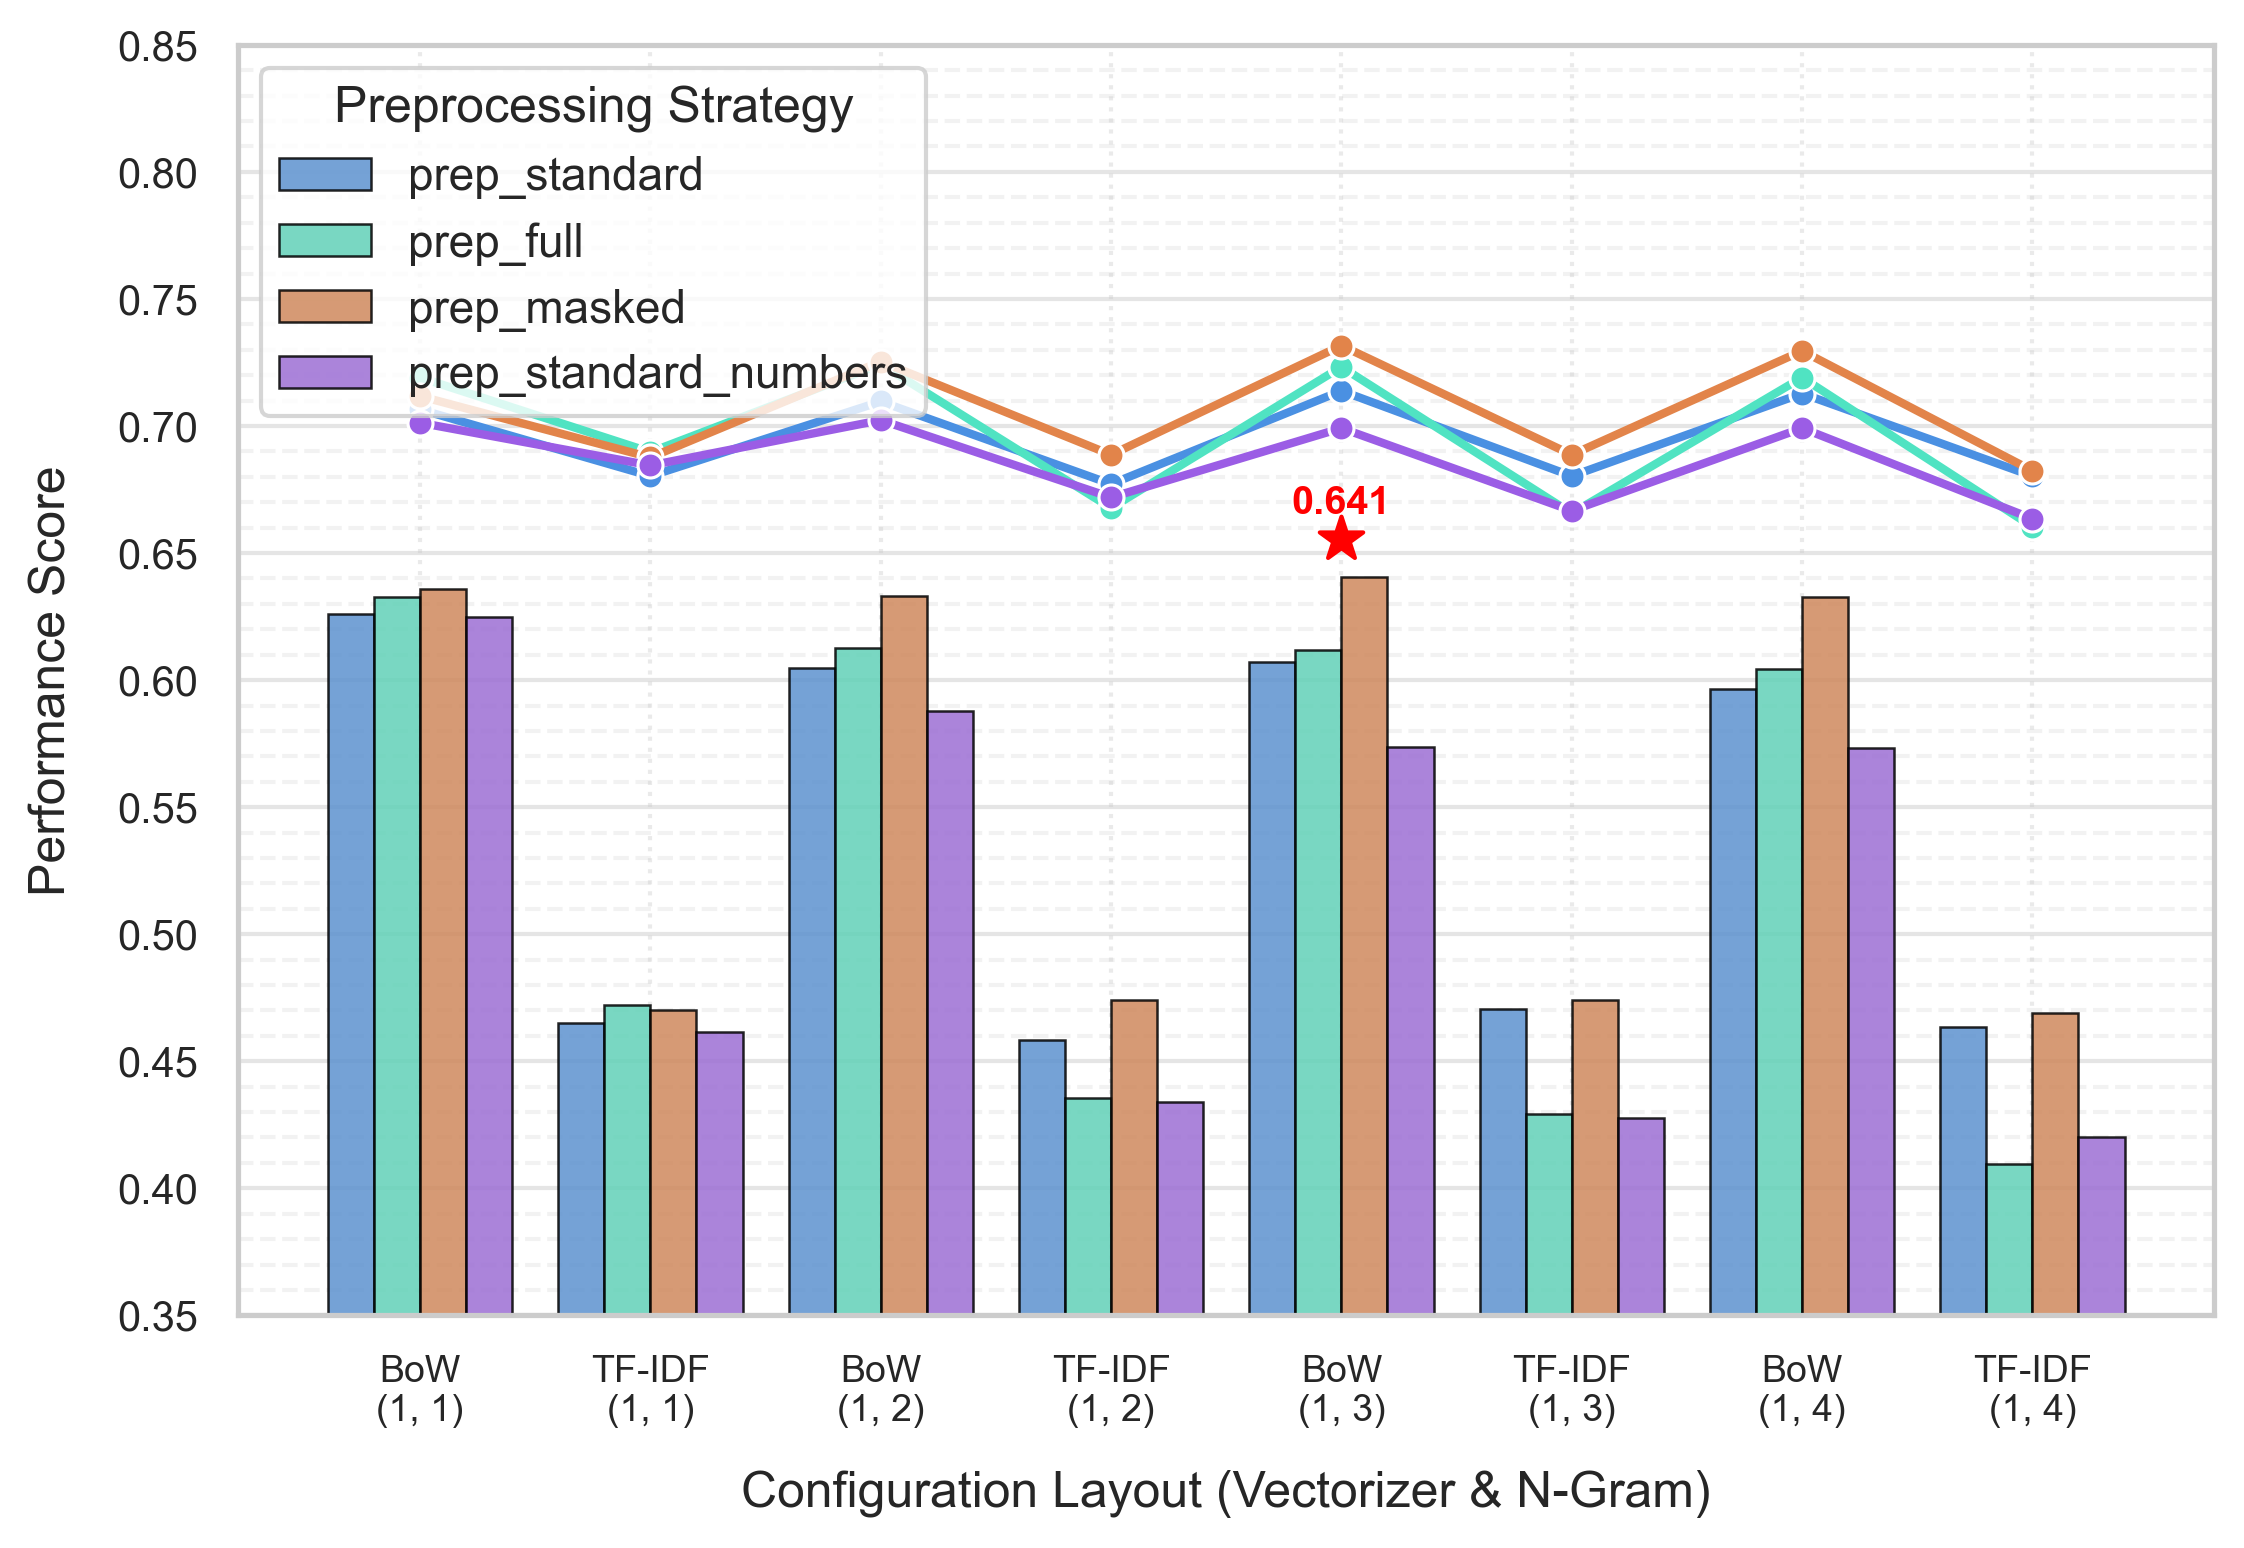
\includegraphics[width=\textwidth]{matrix_naive_bayes_none_(imbalanced).png}
        \caption{Naive Bayes \textbar{} No Sampling}
        \label{fig:nb_none}
    \end{subfigure}
    \hfill
    \begin{subfigure}{0.49\textwidth}
        \centering
        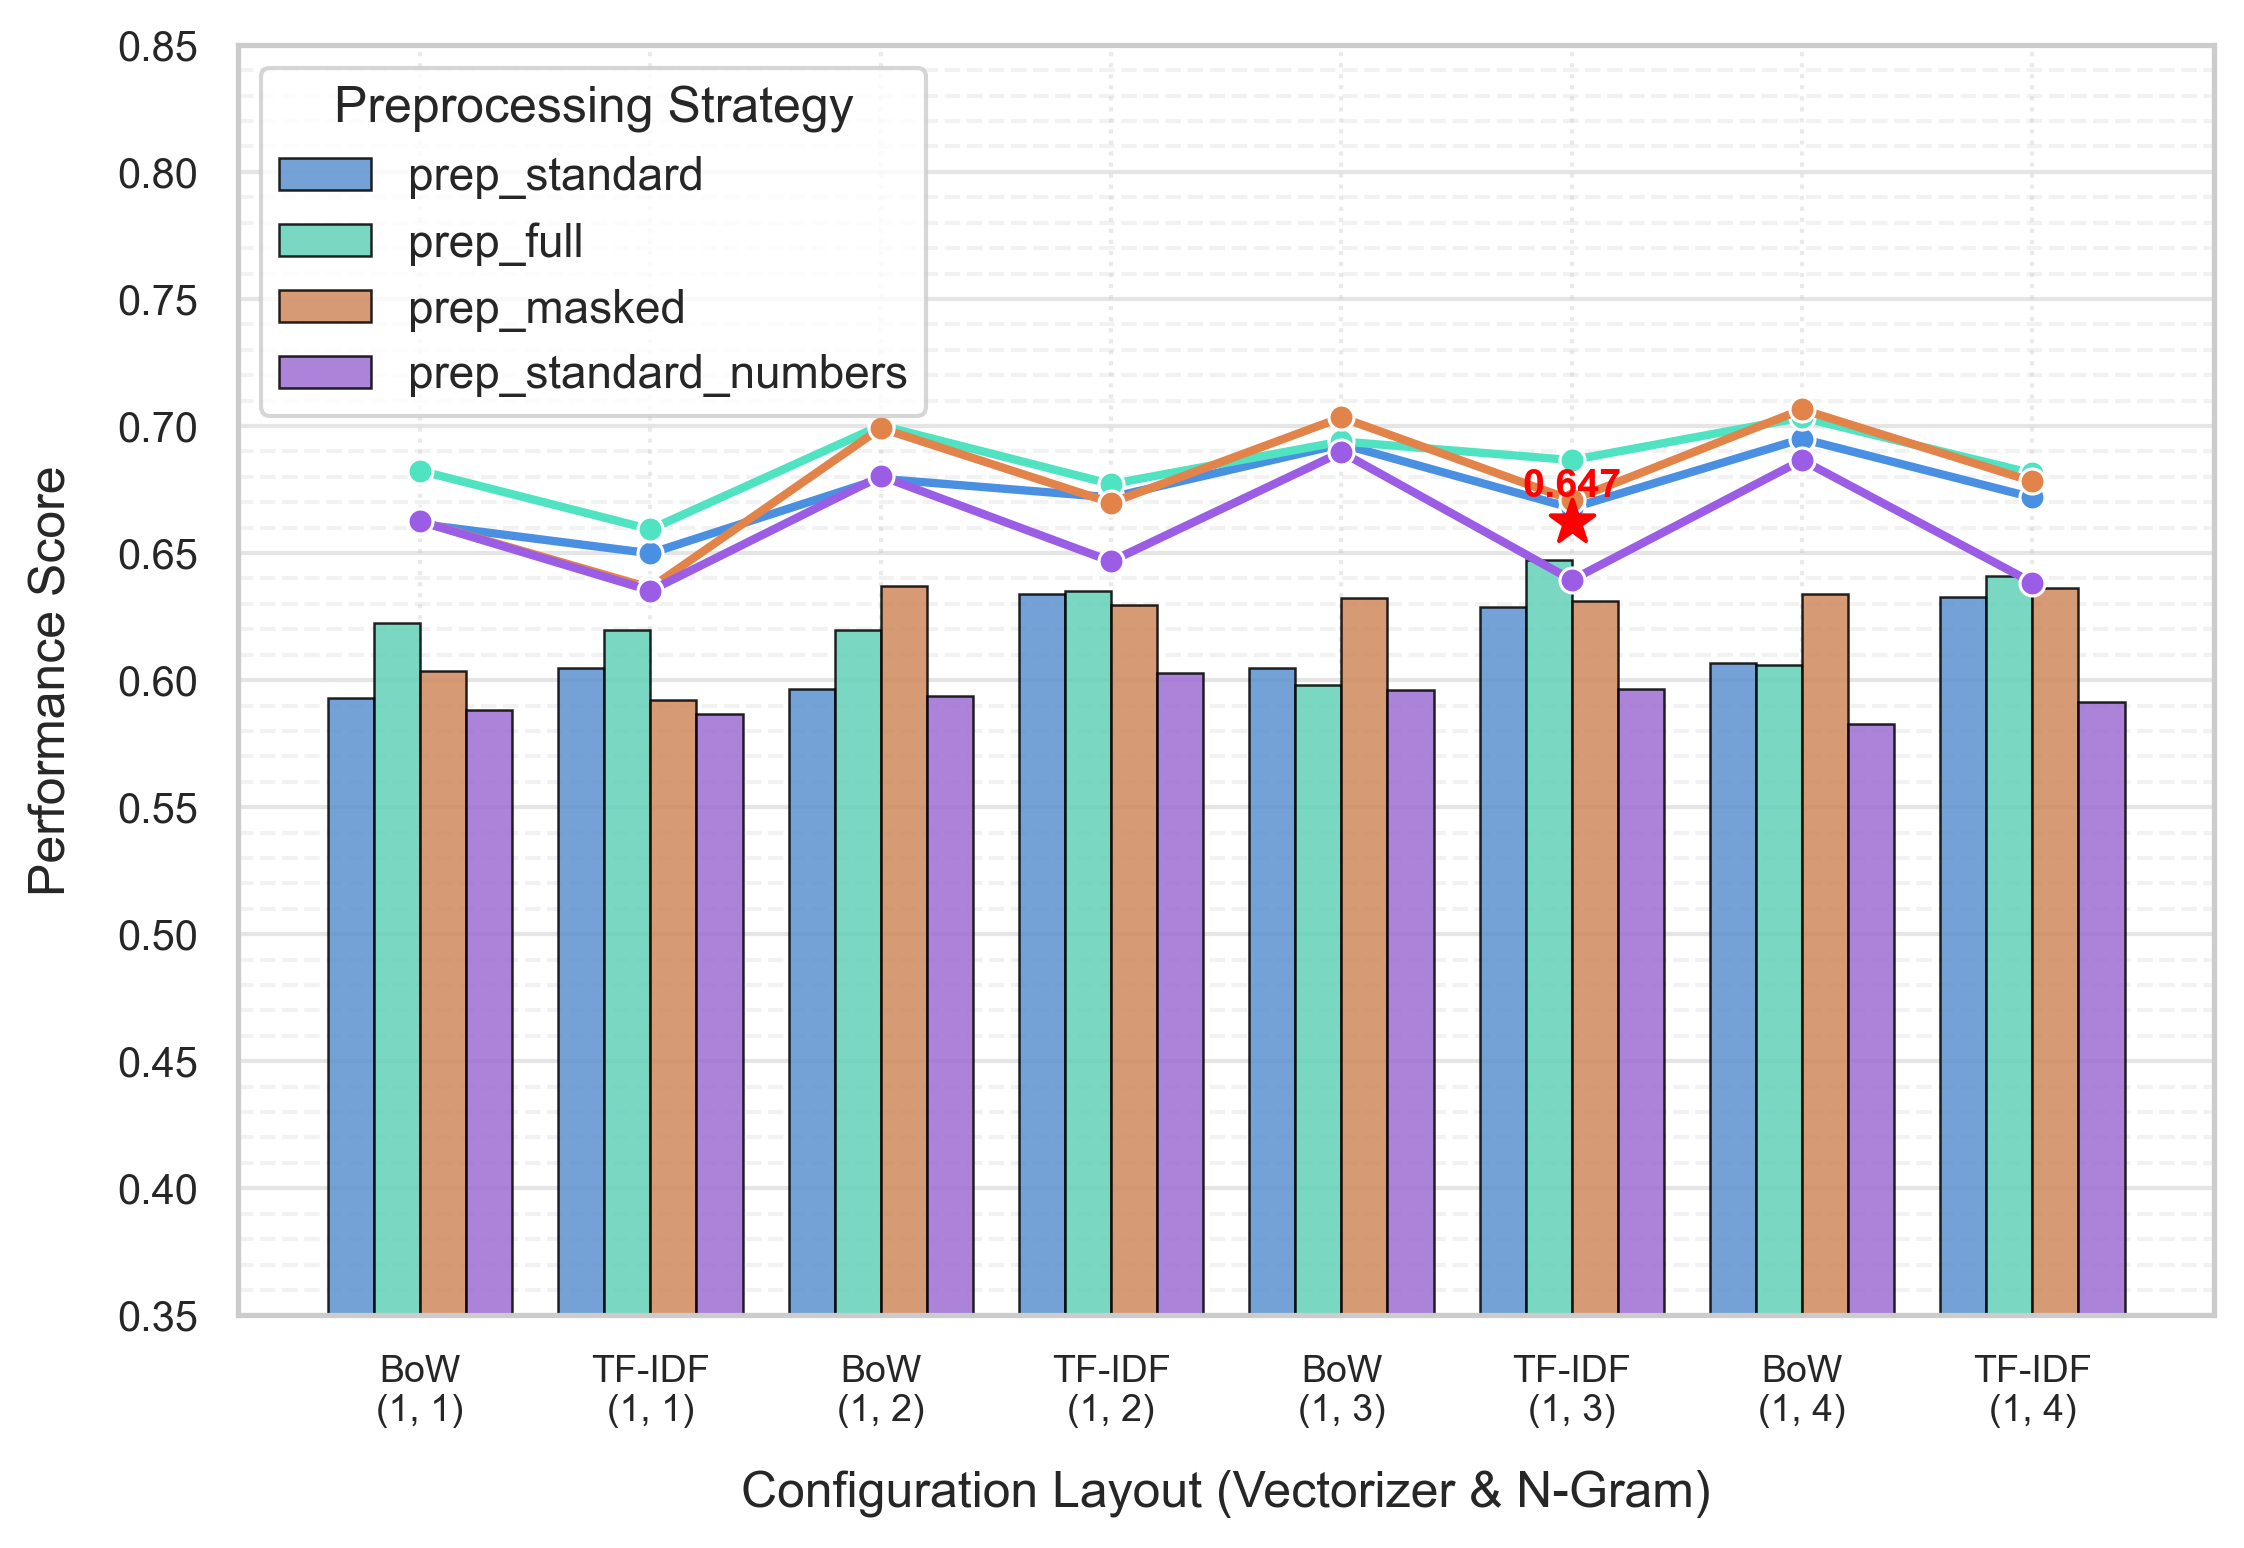
\includegraphics[width=\textwidth]{matrix_naive_bayes_smote_(oversampling).png}
        \caption{Naive Bayes \textbar{} Oversampling}
        \label{fig:nb_over}
    \end{subfigure}

    \vspace{0.4cm}

    \begin{subfigure}{0.49\textwidth}
        \centering
        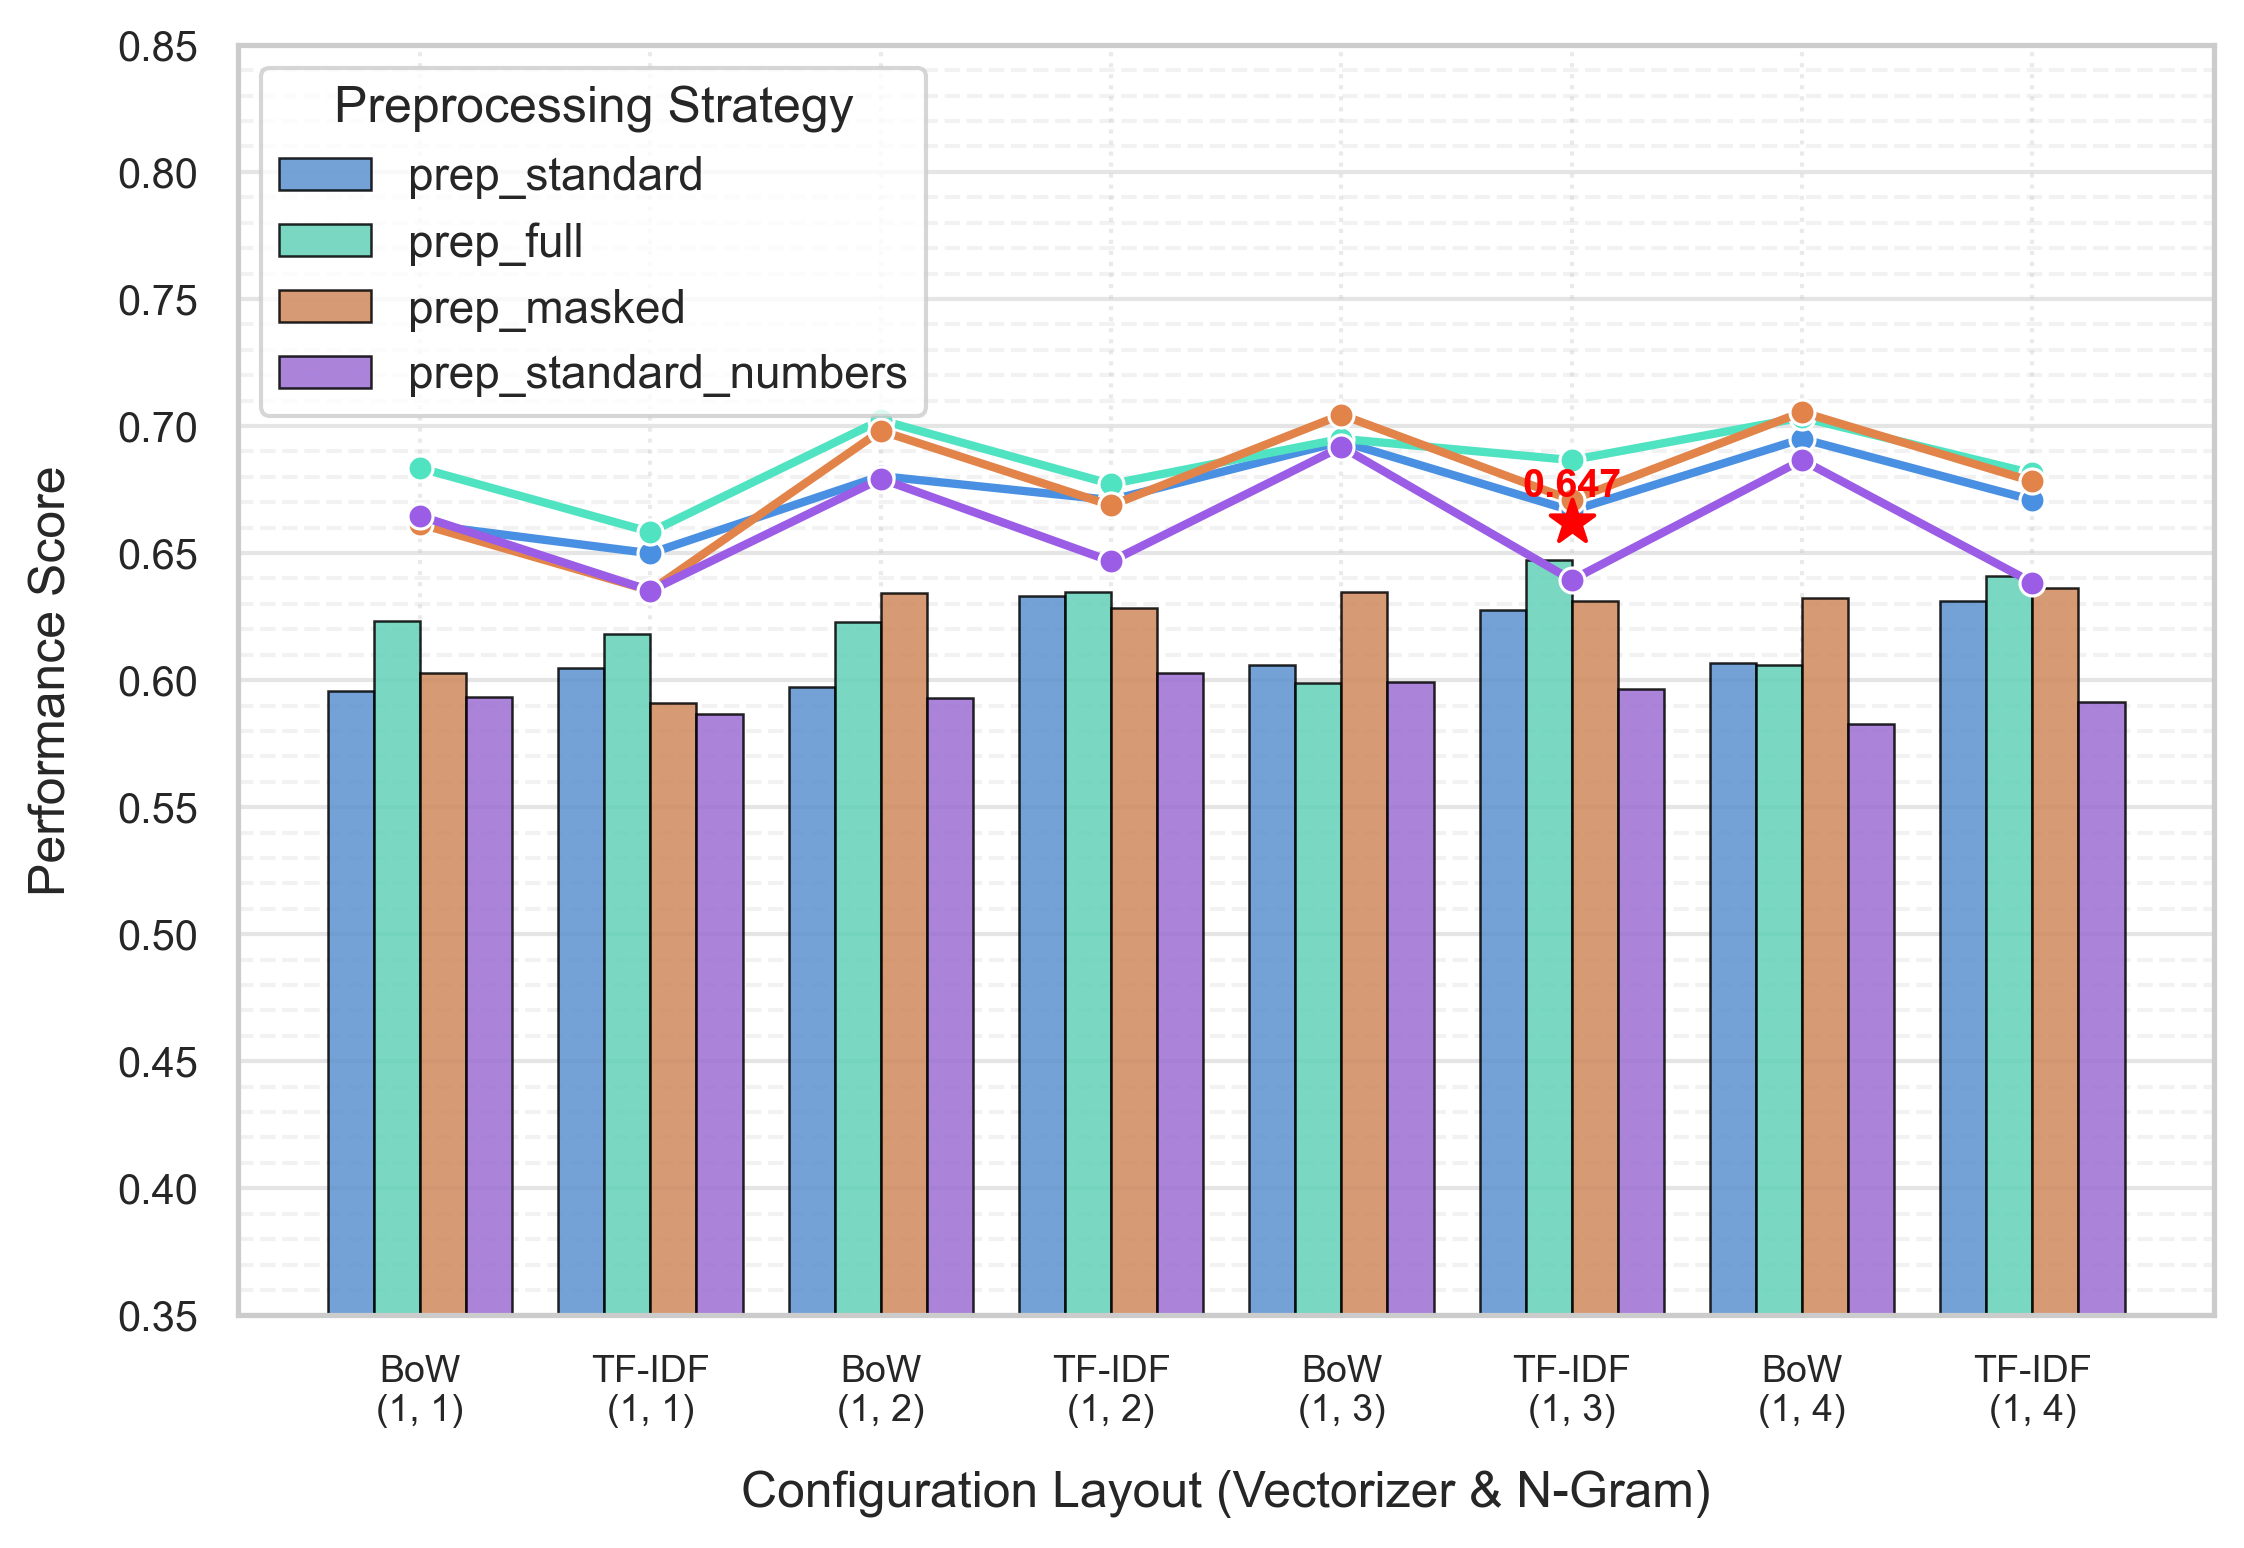
\includegraphics[width=\textwidth]{matrix_naive_bayes_smotetomek_(combined).png}
        \caption{Naive Bayes \textbar{} Under+Oversampling}
        \label{fig:nb_underover}
    \end{subfigure}
    \hfill
    \begin{subfigure}{0.49\textwidth}
        \centering
        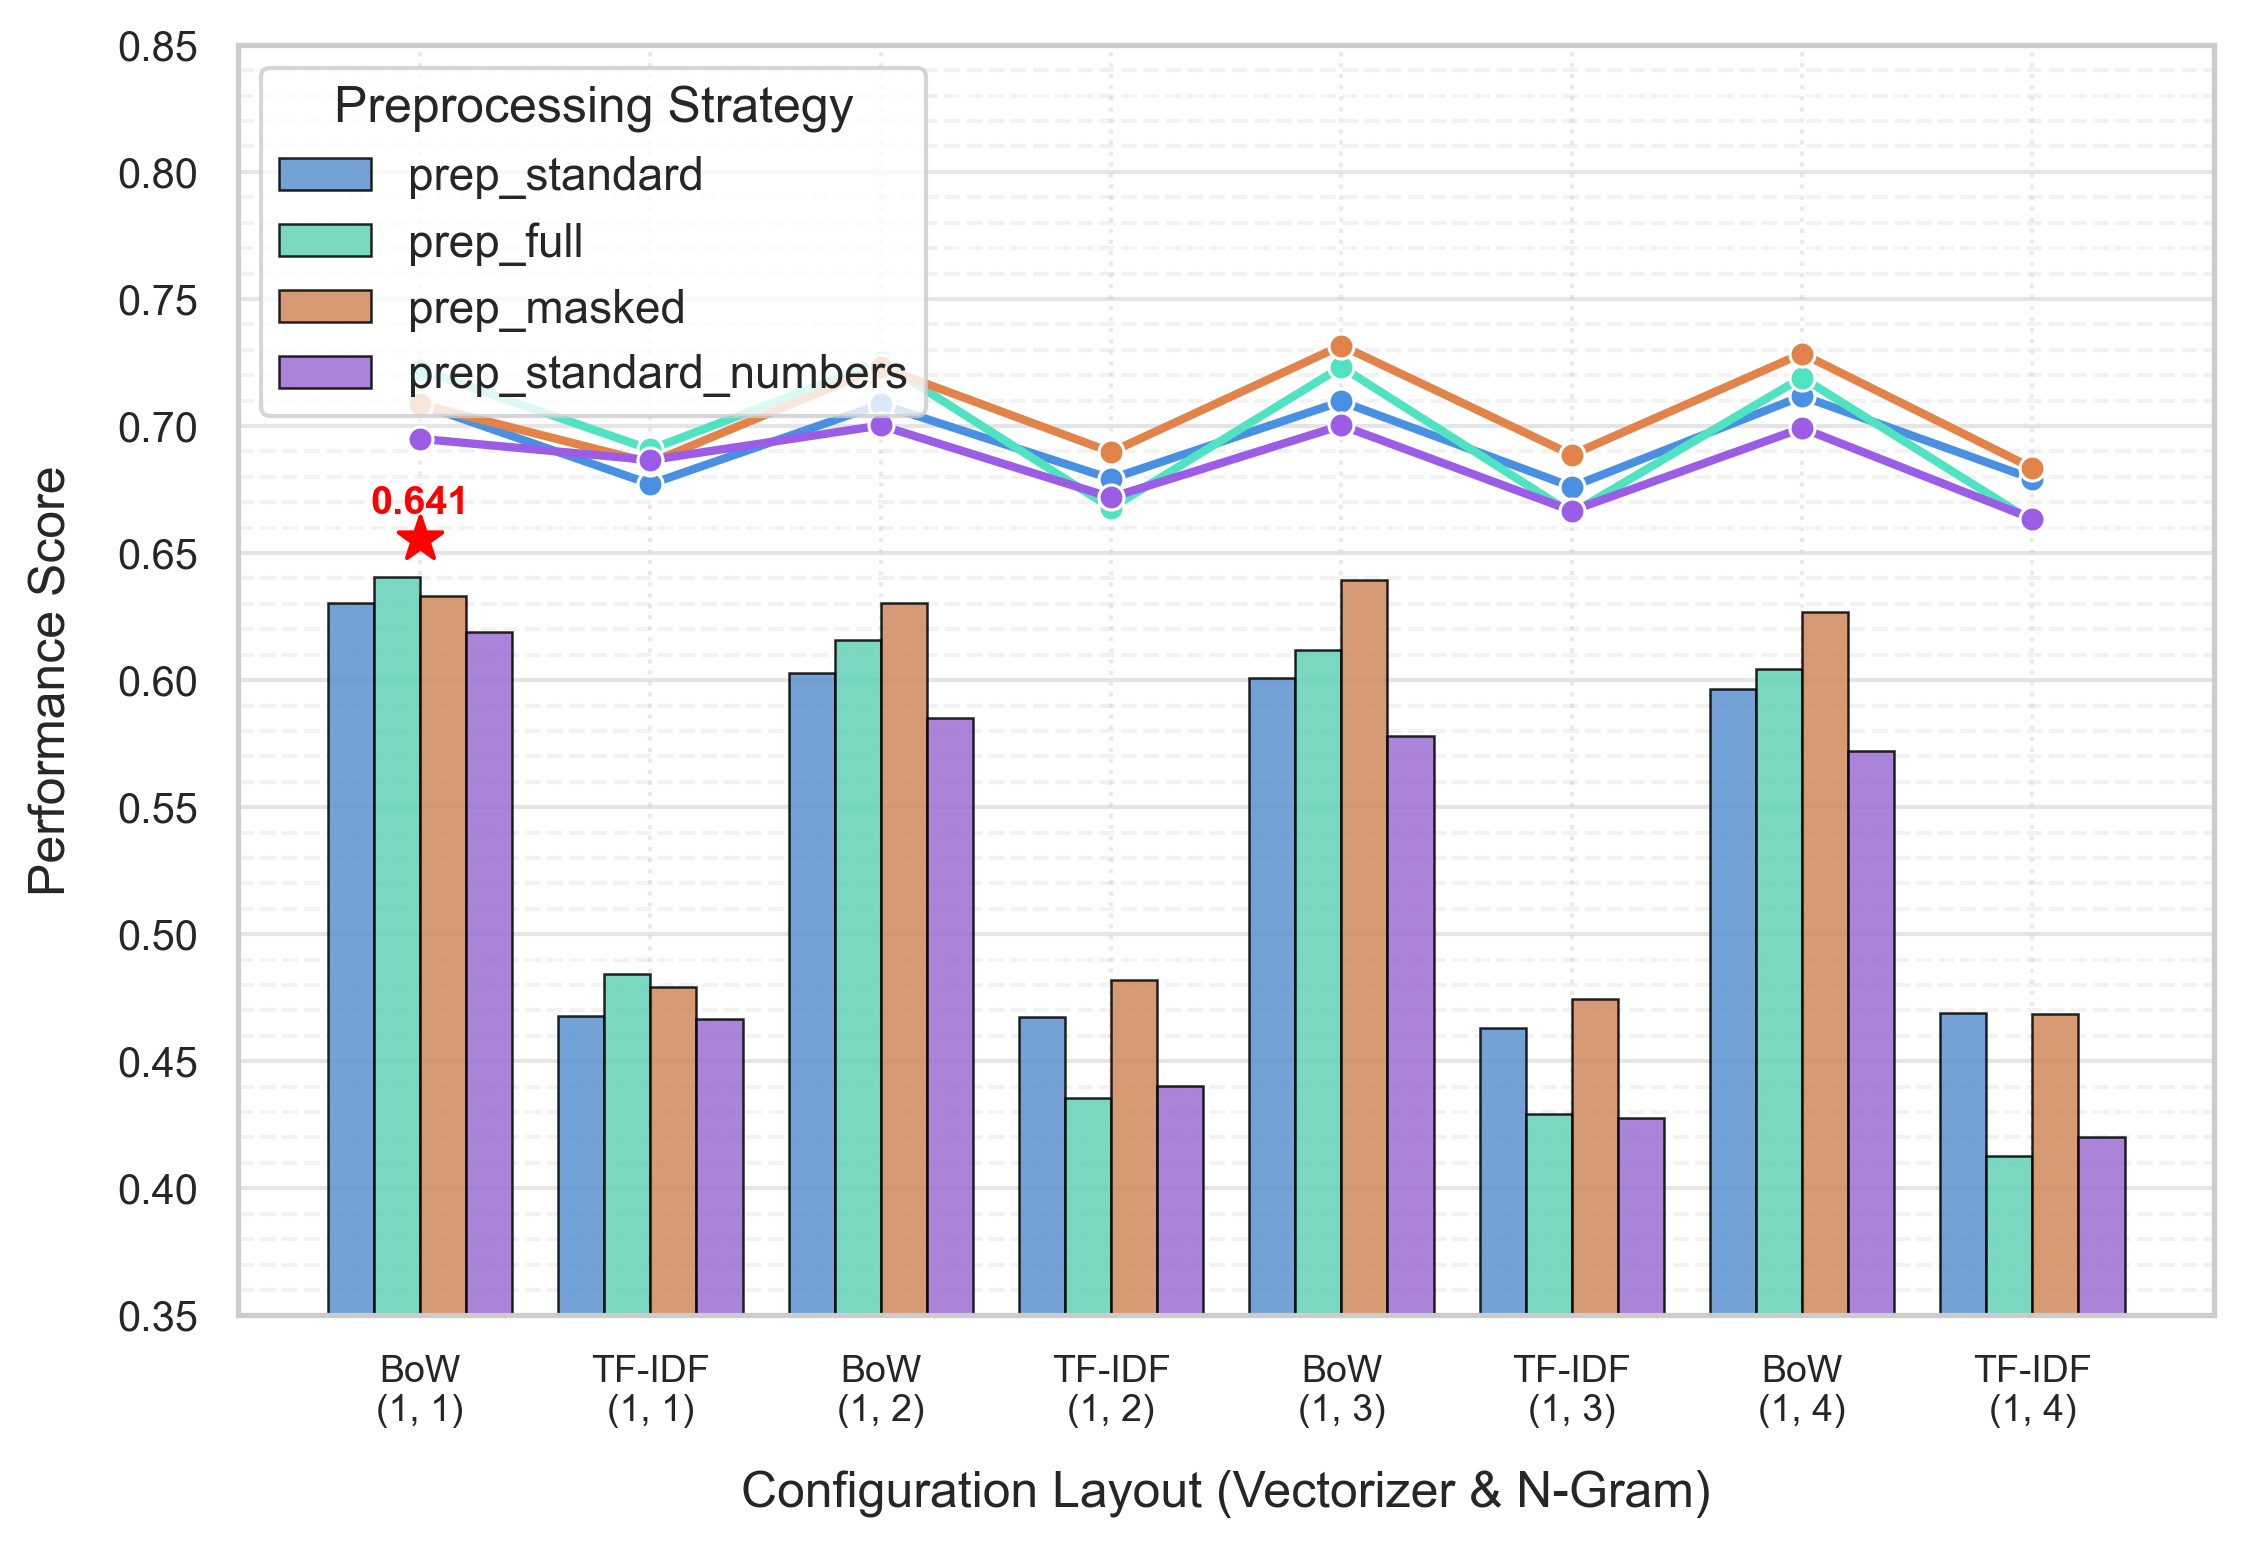
\includegraphics[width=\textwidth]{matrix_naive_bayes_tomek_(undersampling).png}
        \caption{Naive Bayes \textbar{} Undersampling}
        \label{fig:nb_under}
    \end{subfigure}
    \caption{Grand Performance Matrix (Part 1): \textsc{mnb} classification topologies across varying dataset oversampling techniques.}
    \label{fig:grand_matrix_part1}
\end{figure}

\begin{figure}[H]
    \centering
    \begin{subfigure}{0.49\textwidth}
        \centering
        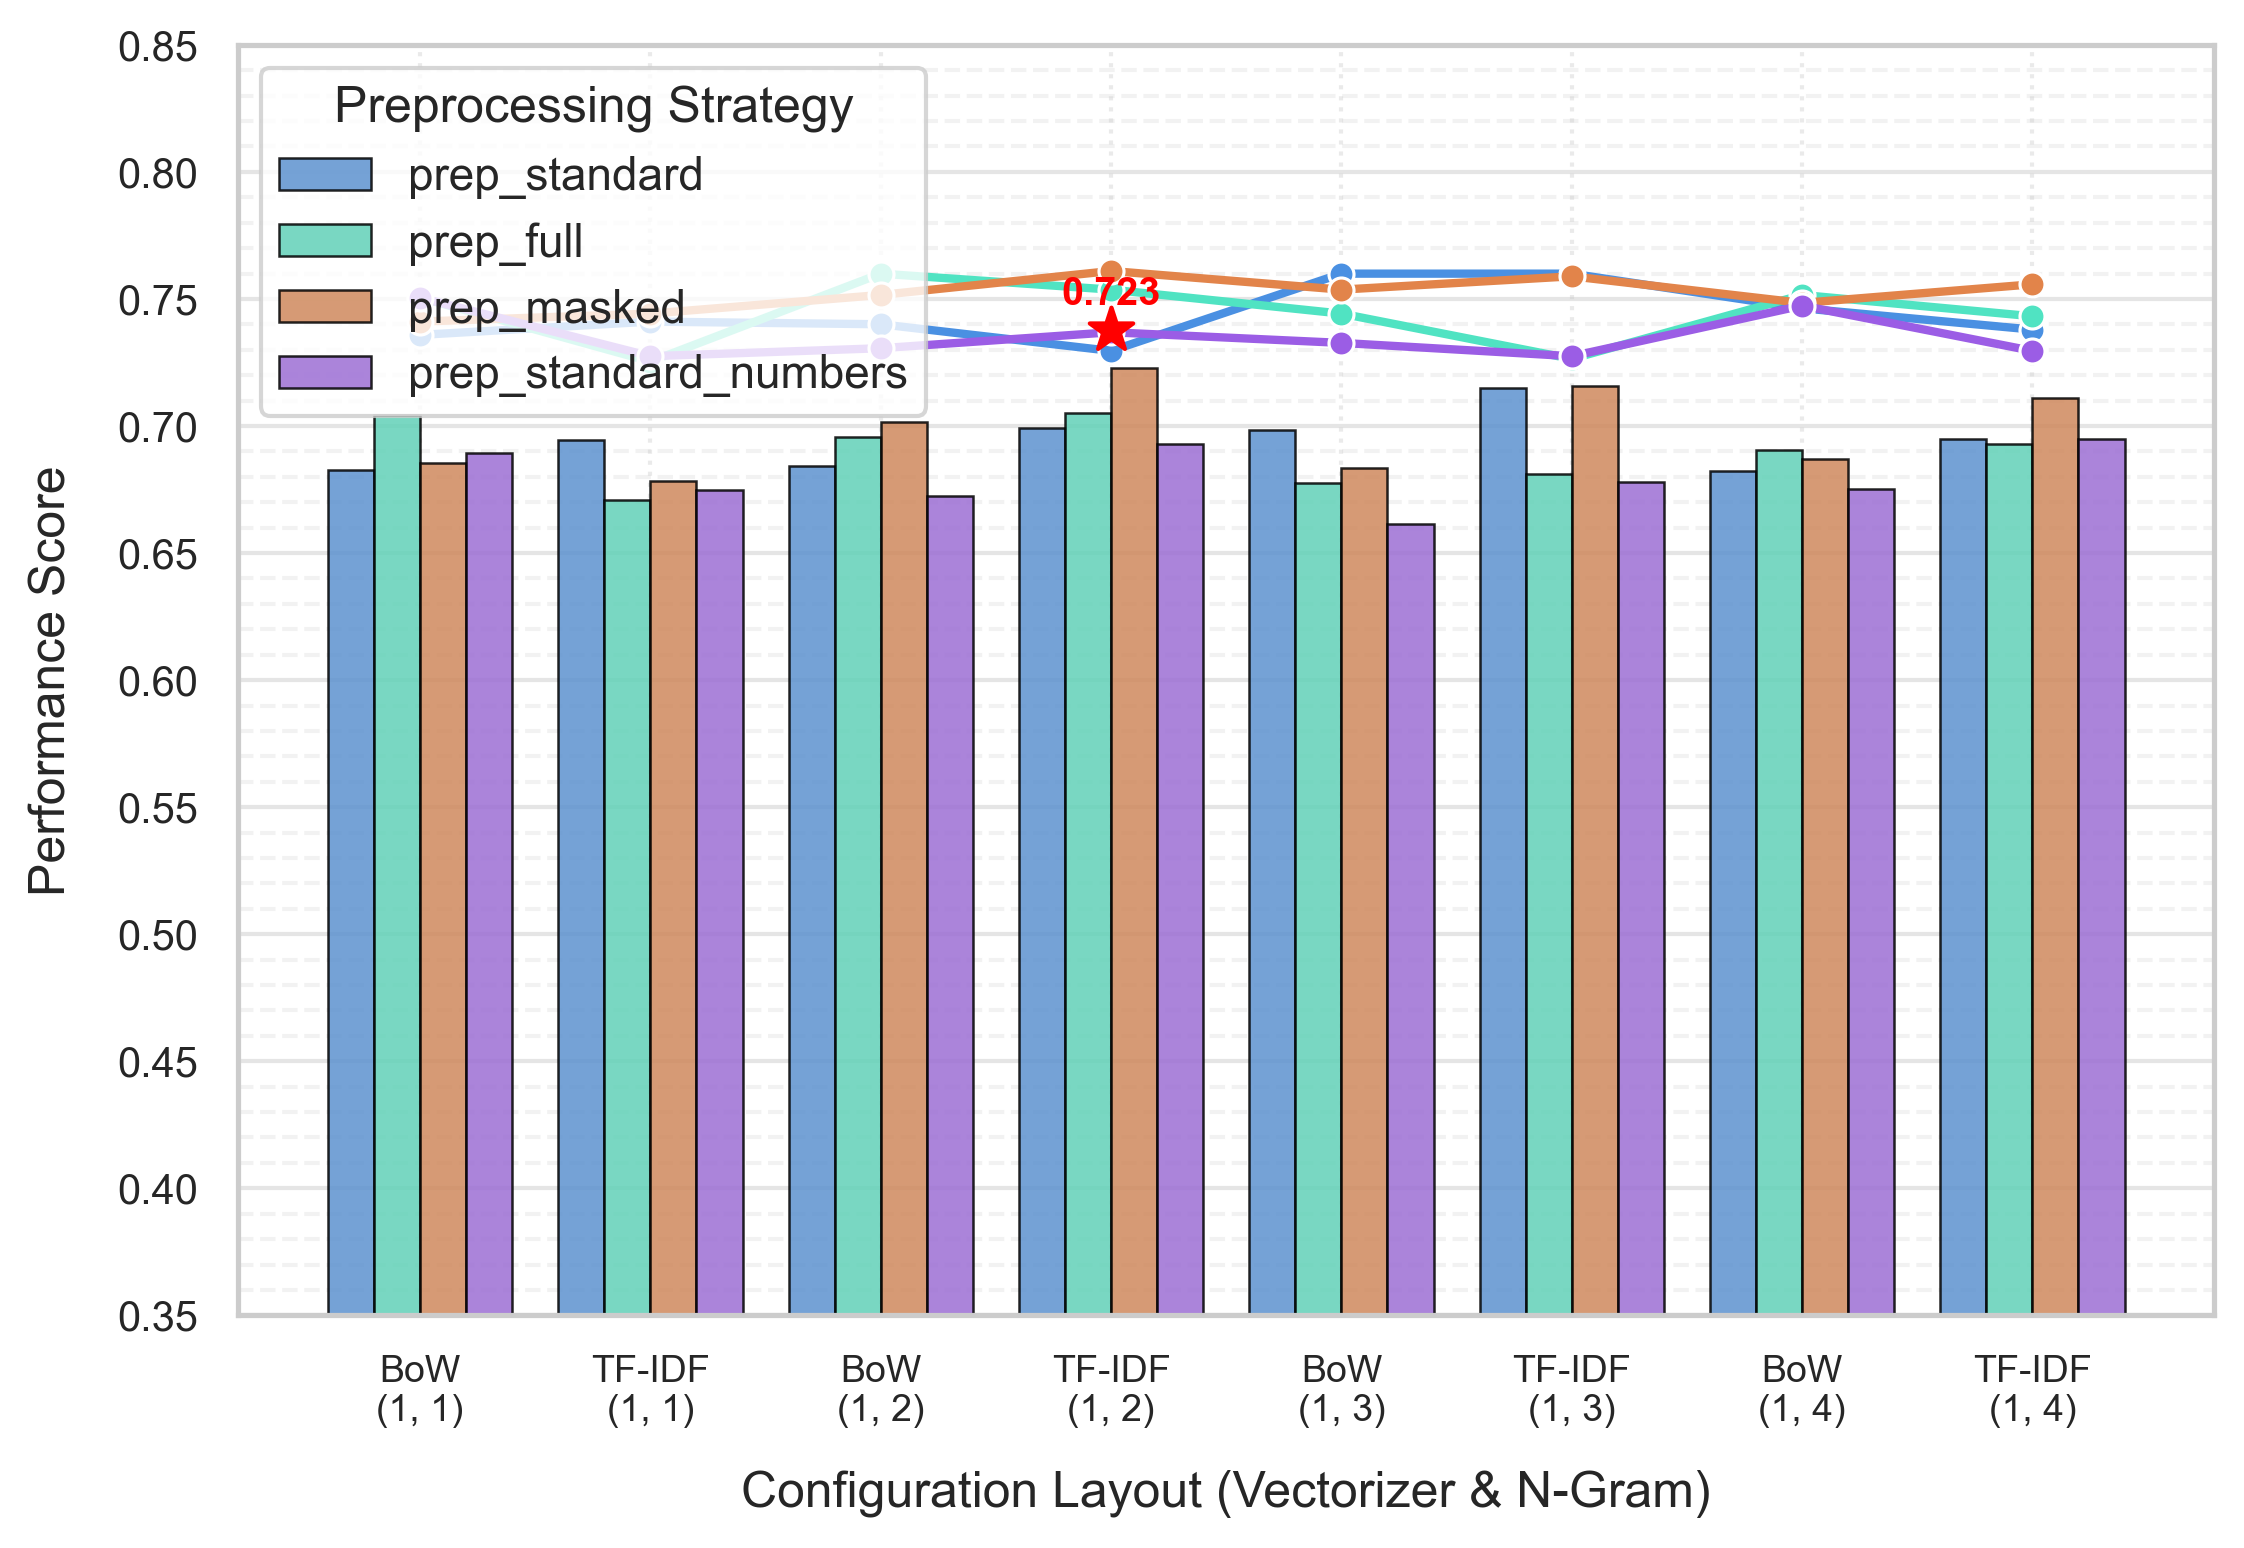
\includegraphics[width=\textwidth]{matrix_ffnn_updated_none_(imbalanced).png}
        \caption{FFNN \textbar{} No Sampling}
        \label{fig:ffnn_none}
    \end{subfigure}
    \hfill
    \begin{subfigure}{0.49\textwidth}
        \centering
        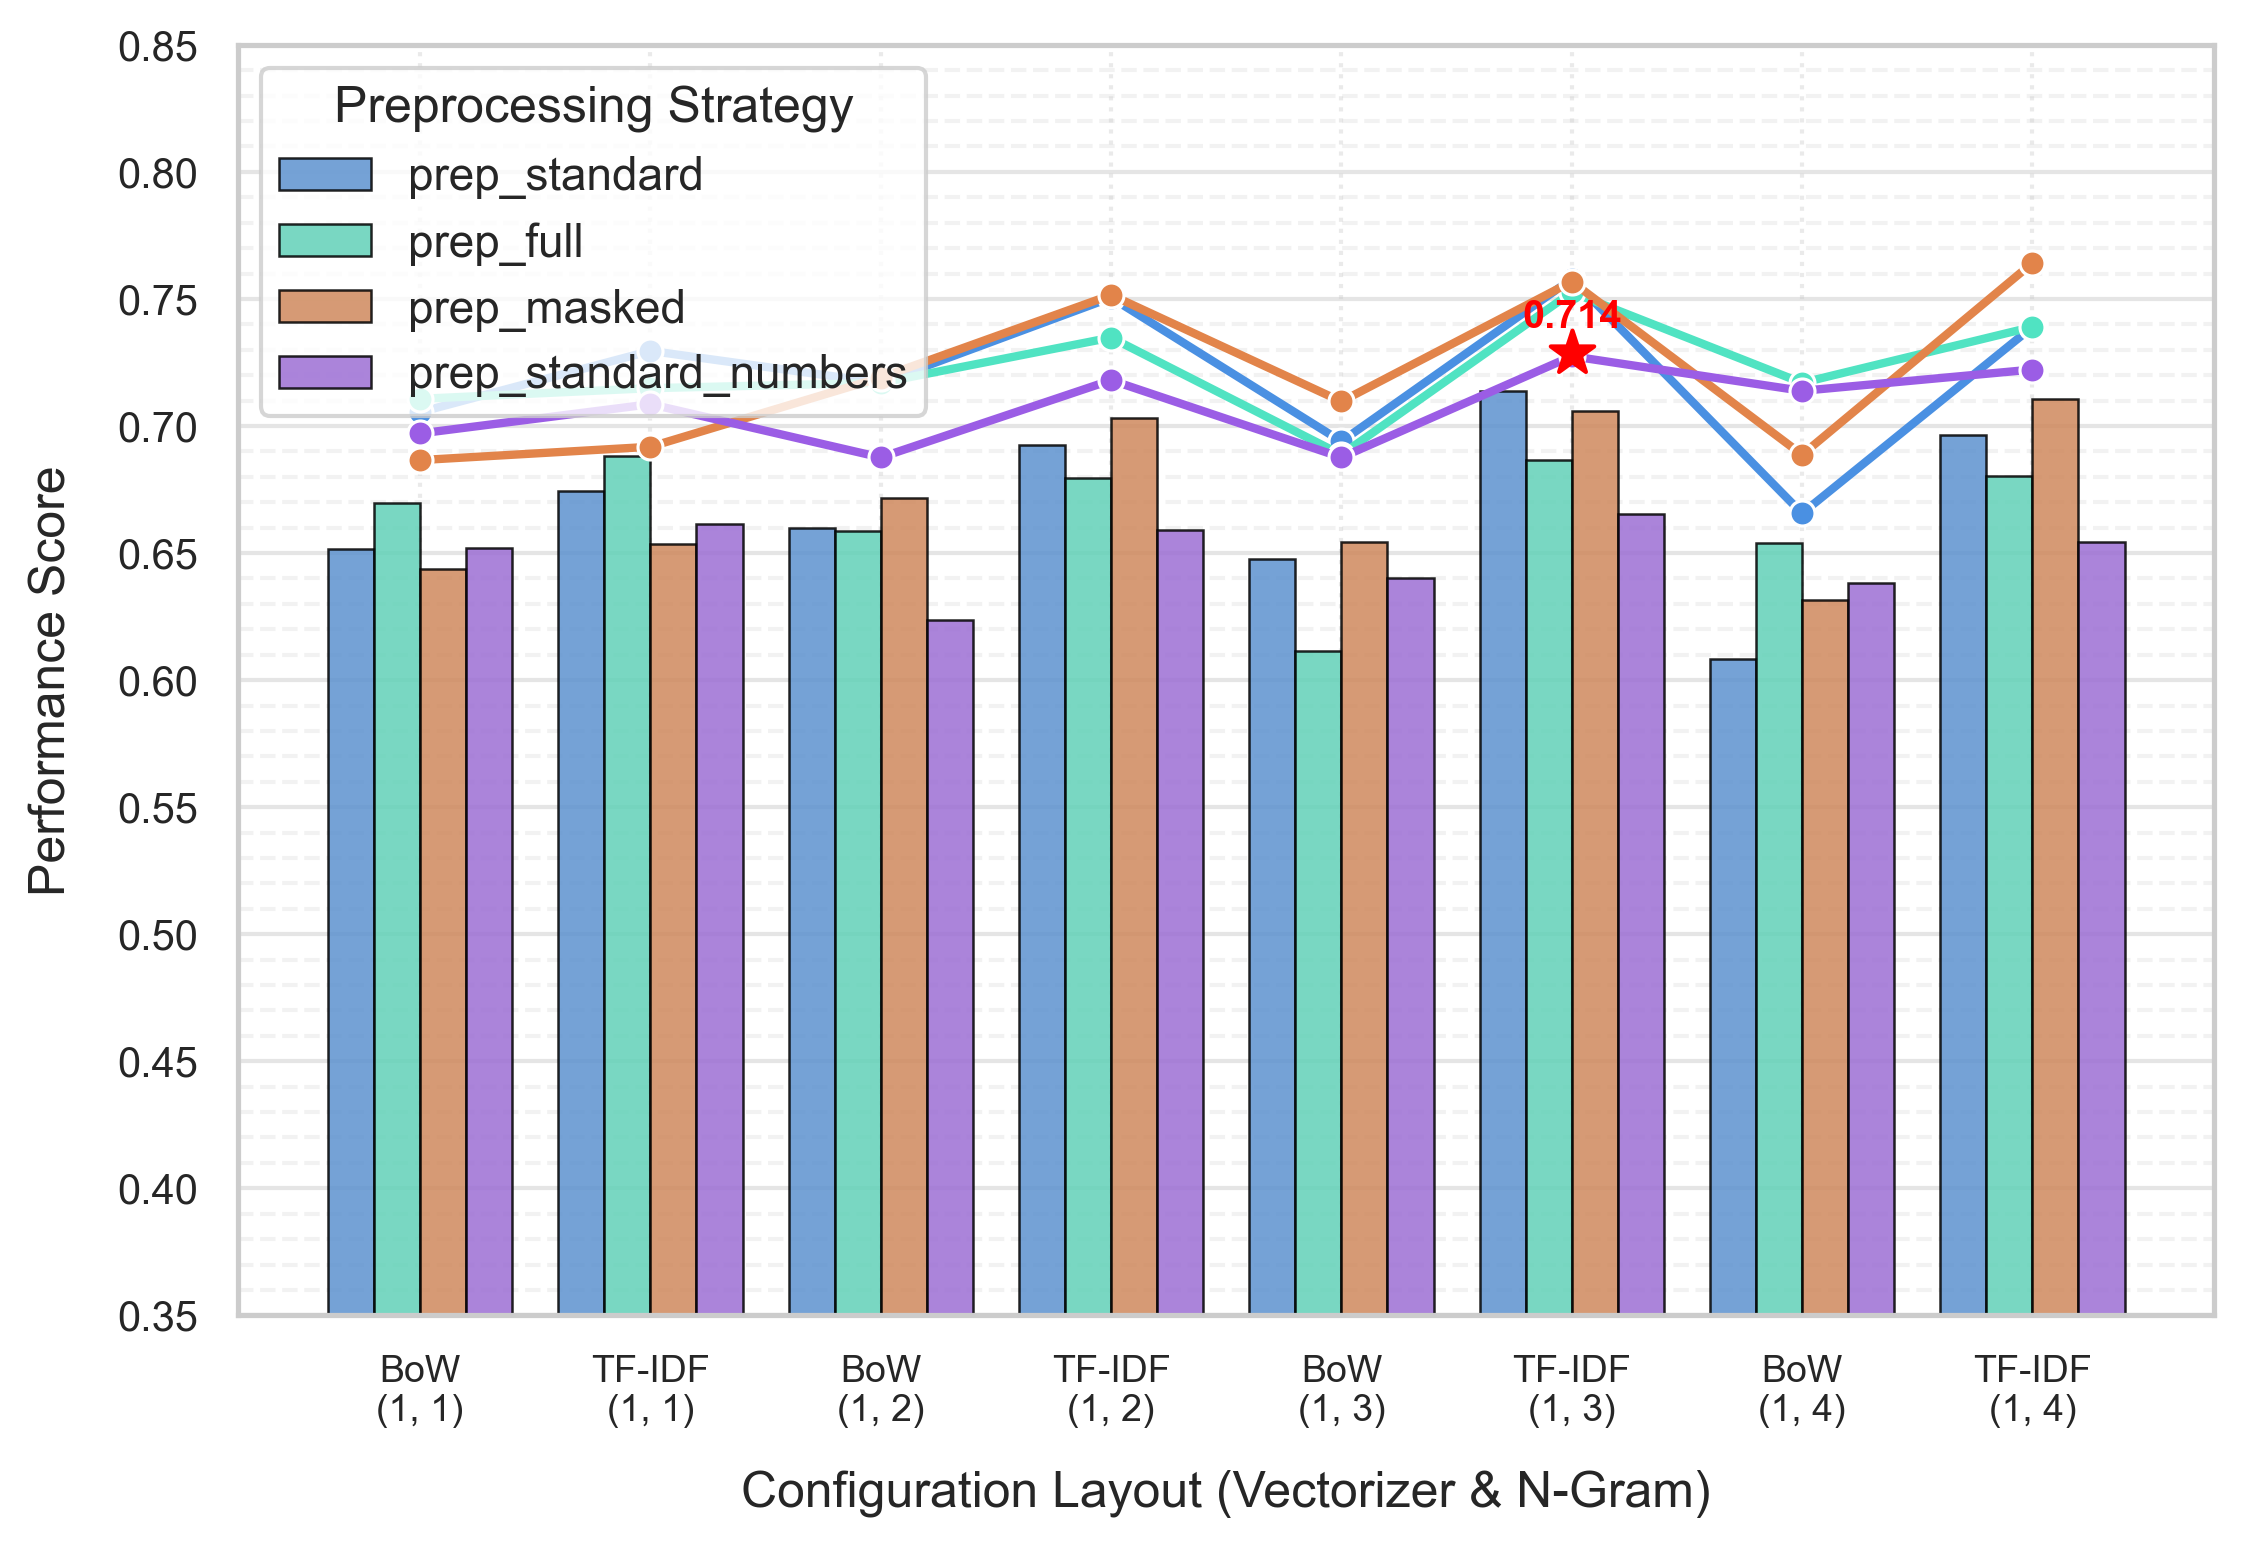
\includegraphics[width=\textwidth]{matrix_ffnn_updated_smote_(oversampling).png}
        \caption{FFNN \textbar{} Over+Undersampling}
        \label{fig:ffnn_over}
    \end{subfigure}

    \vspace{0.4cm}

    \begin{subfigure}{0.49\textwidth}
        \centering
        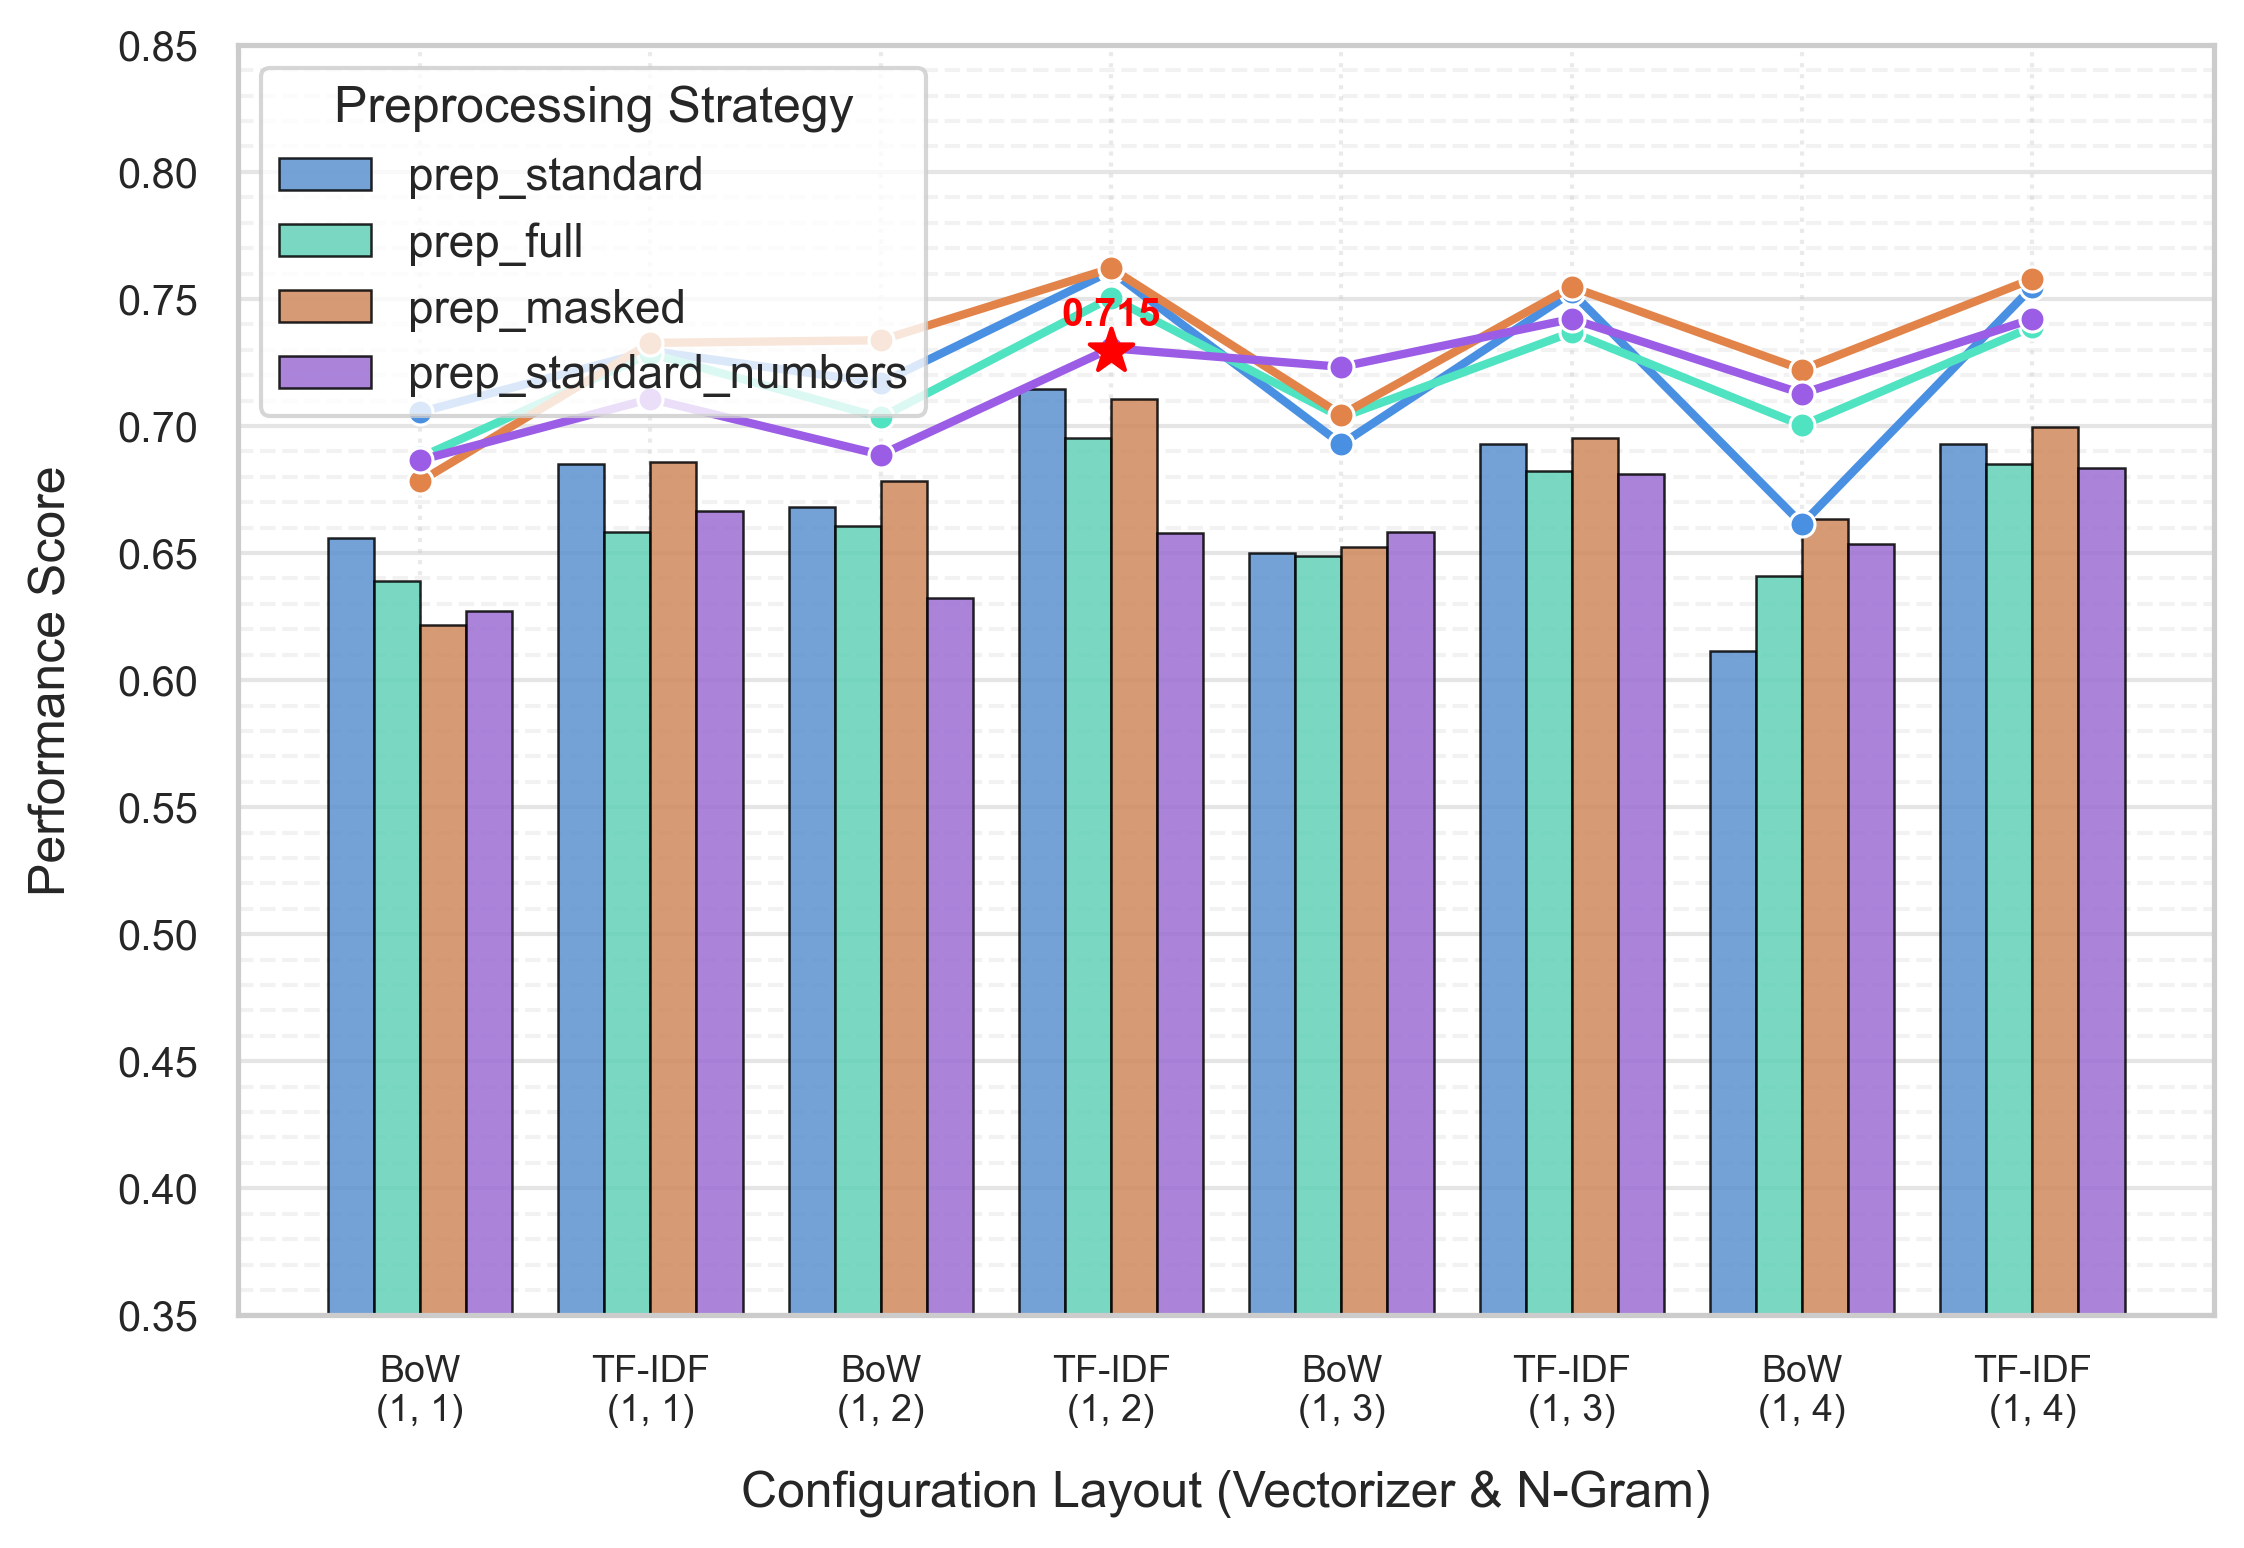
\includegraphics[width=\textwidth]{matrix_ffnn_updated_smotetomek_(combined).png}
        \caption{FFNN \textbar{} Under+Oversampling}
        \label{fig:ffnn_underover}
    \end{subfigure}
    \hfill
    \begin{subfigure}{0.49\textwidth}
        \centering
        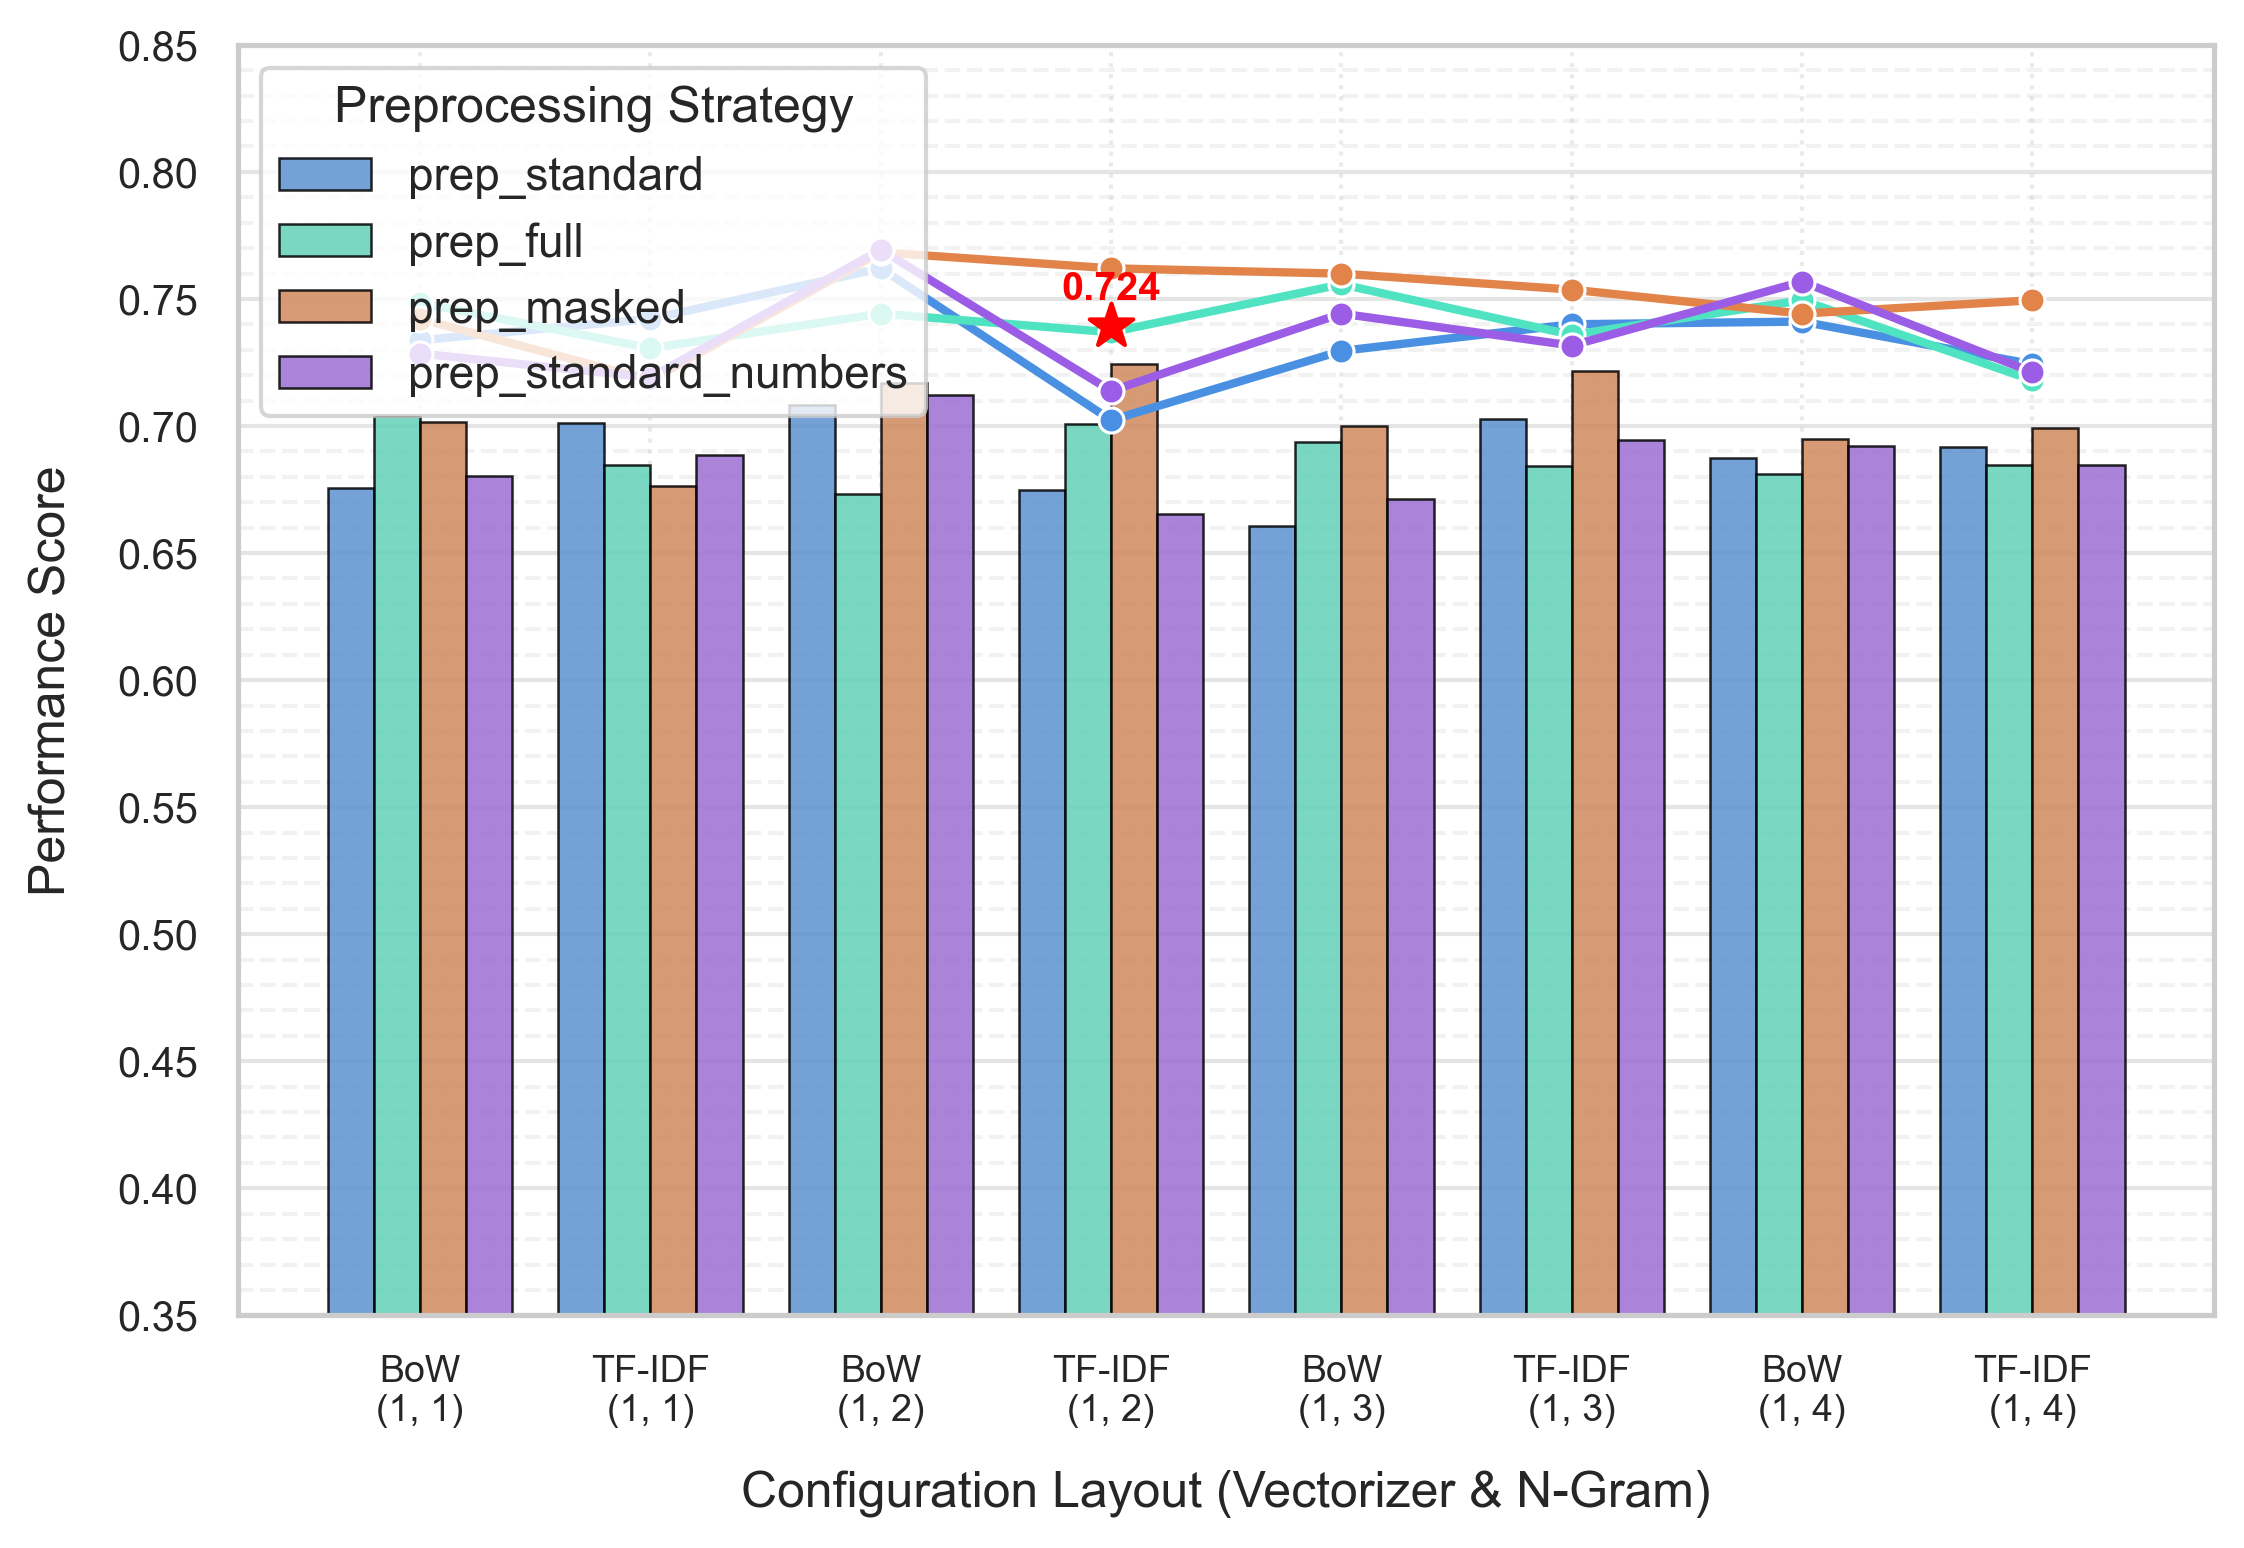
\includegraphics[width=\textwidth]{matrix_ffnn_updated_tomek_(undersampling).png}
        \caption{FFNN  \textbar{} Undersampling}
        \label{fig:ffnn_under}
    \end{subfigure}
    \caption{Grand Performance Matrix (Part 2): End-to-end evaluation parsing performance limits across \textsc{mnb} extensions and Feed-Forward Neural Architectures.}
    \label{fig:grand_matrix_part2}
\end{figure}

\section{Confusion Matrix - Bayes + FFNN}
\label{app:confusion_matrix}

\begin{figure}[H]
    \centering
    \begin{subfigure}{0.49\textwidth}
        \centering
        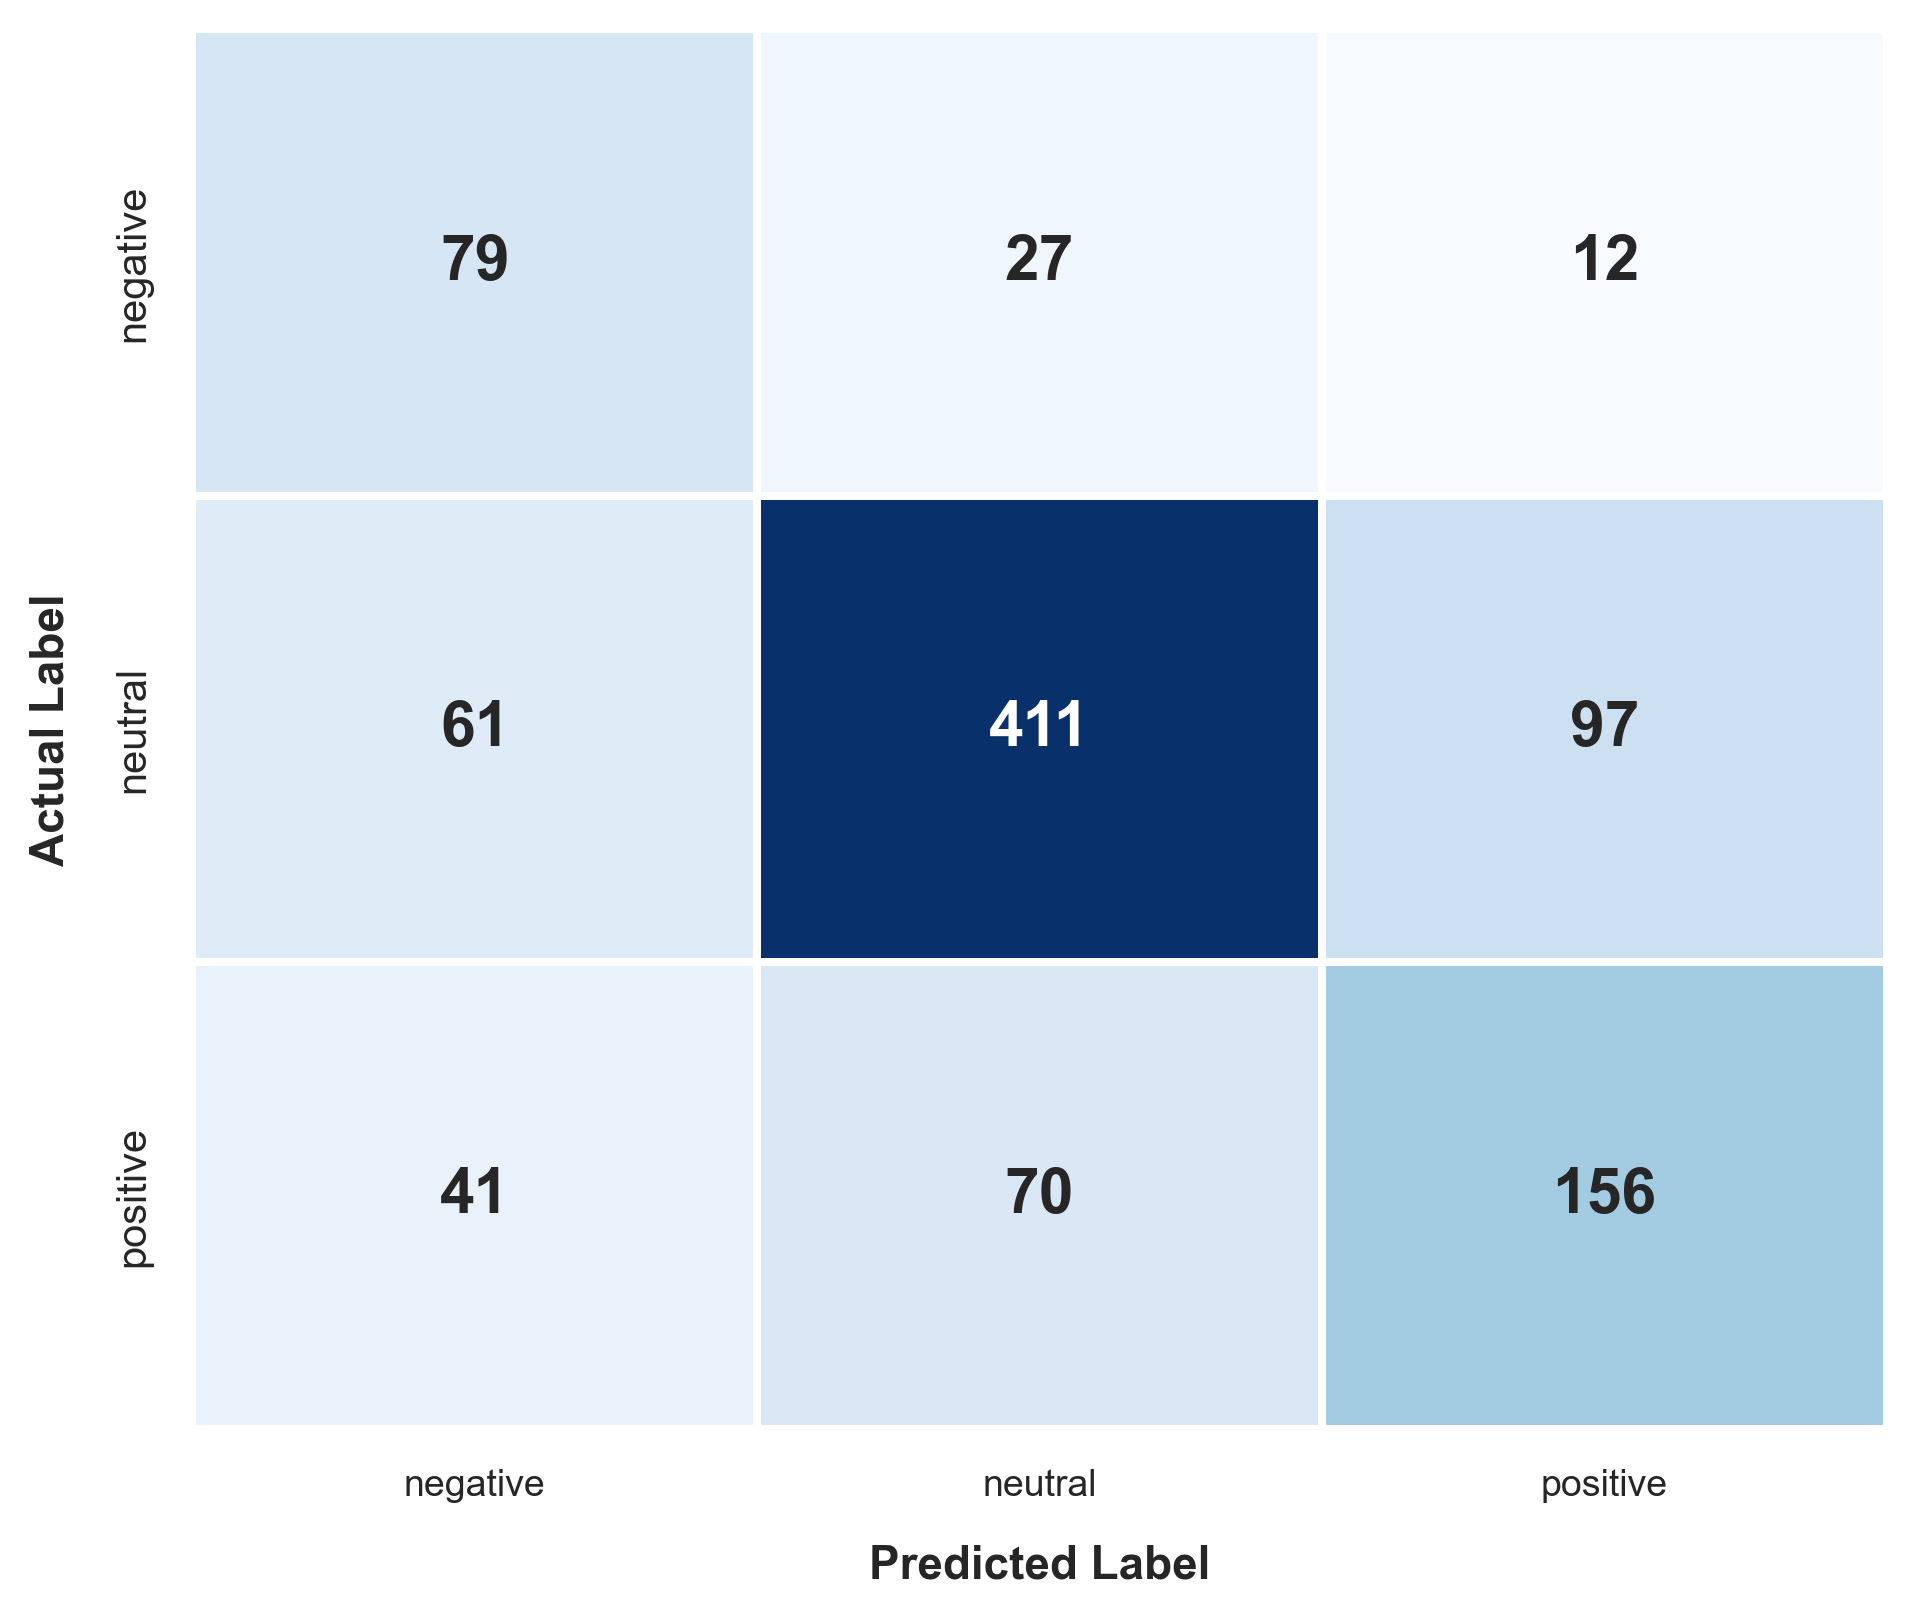
\includegraphics[width=\textwidth]{confusion_matrix_naive_bayes.png}
        \caption*{\textbf{Best Config: \textsc{mnb} + \textsc{bow}}\\
        Strategy: ($\mathcal{S}_3$) \textbar{} $n$-Gram: (1, 3) \textbar{} SMOTE (Oversamlping) \\
        Macro-$F_1$: 0.65}
        \label{fig:best_cm_nb}
    \end{subfigure}
    \hfill
    \begin{subfigure}{0.49\textwidth}
        \centering
        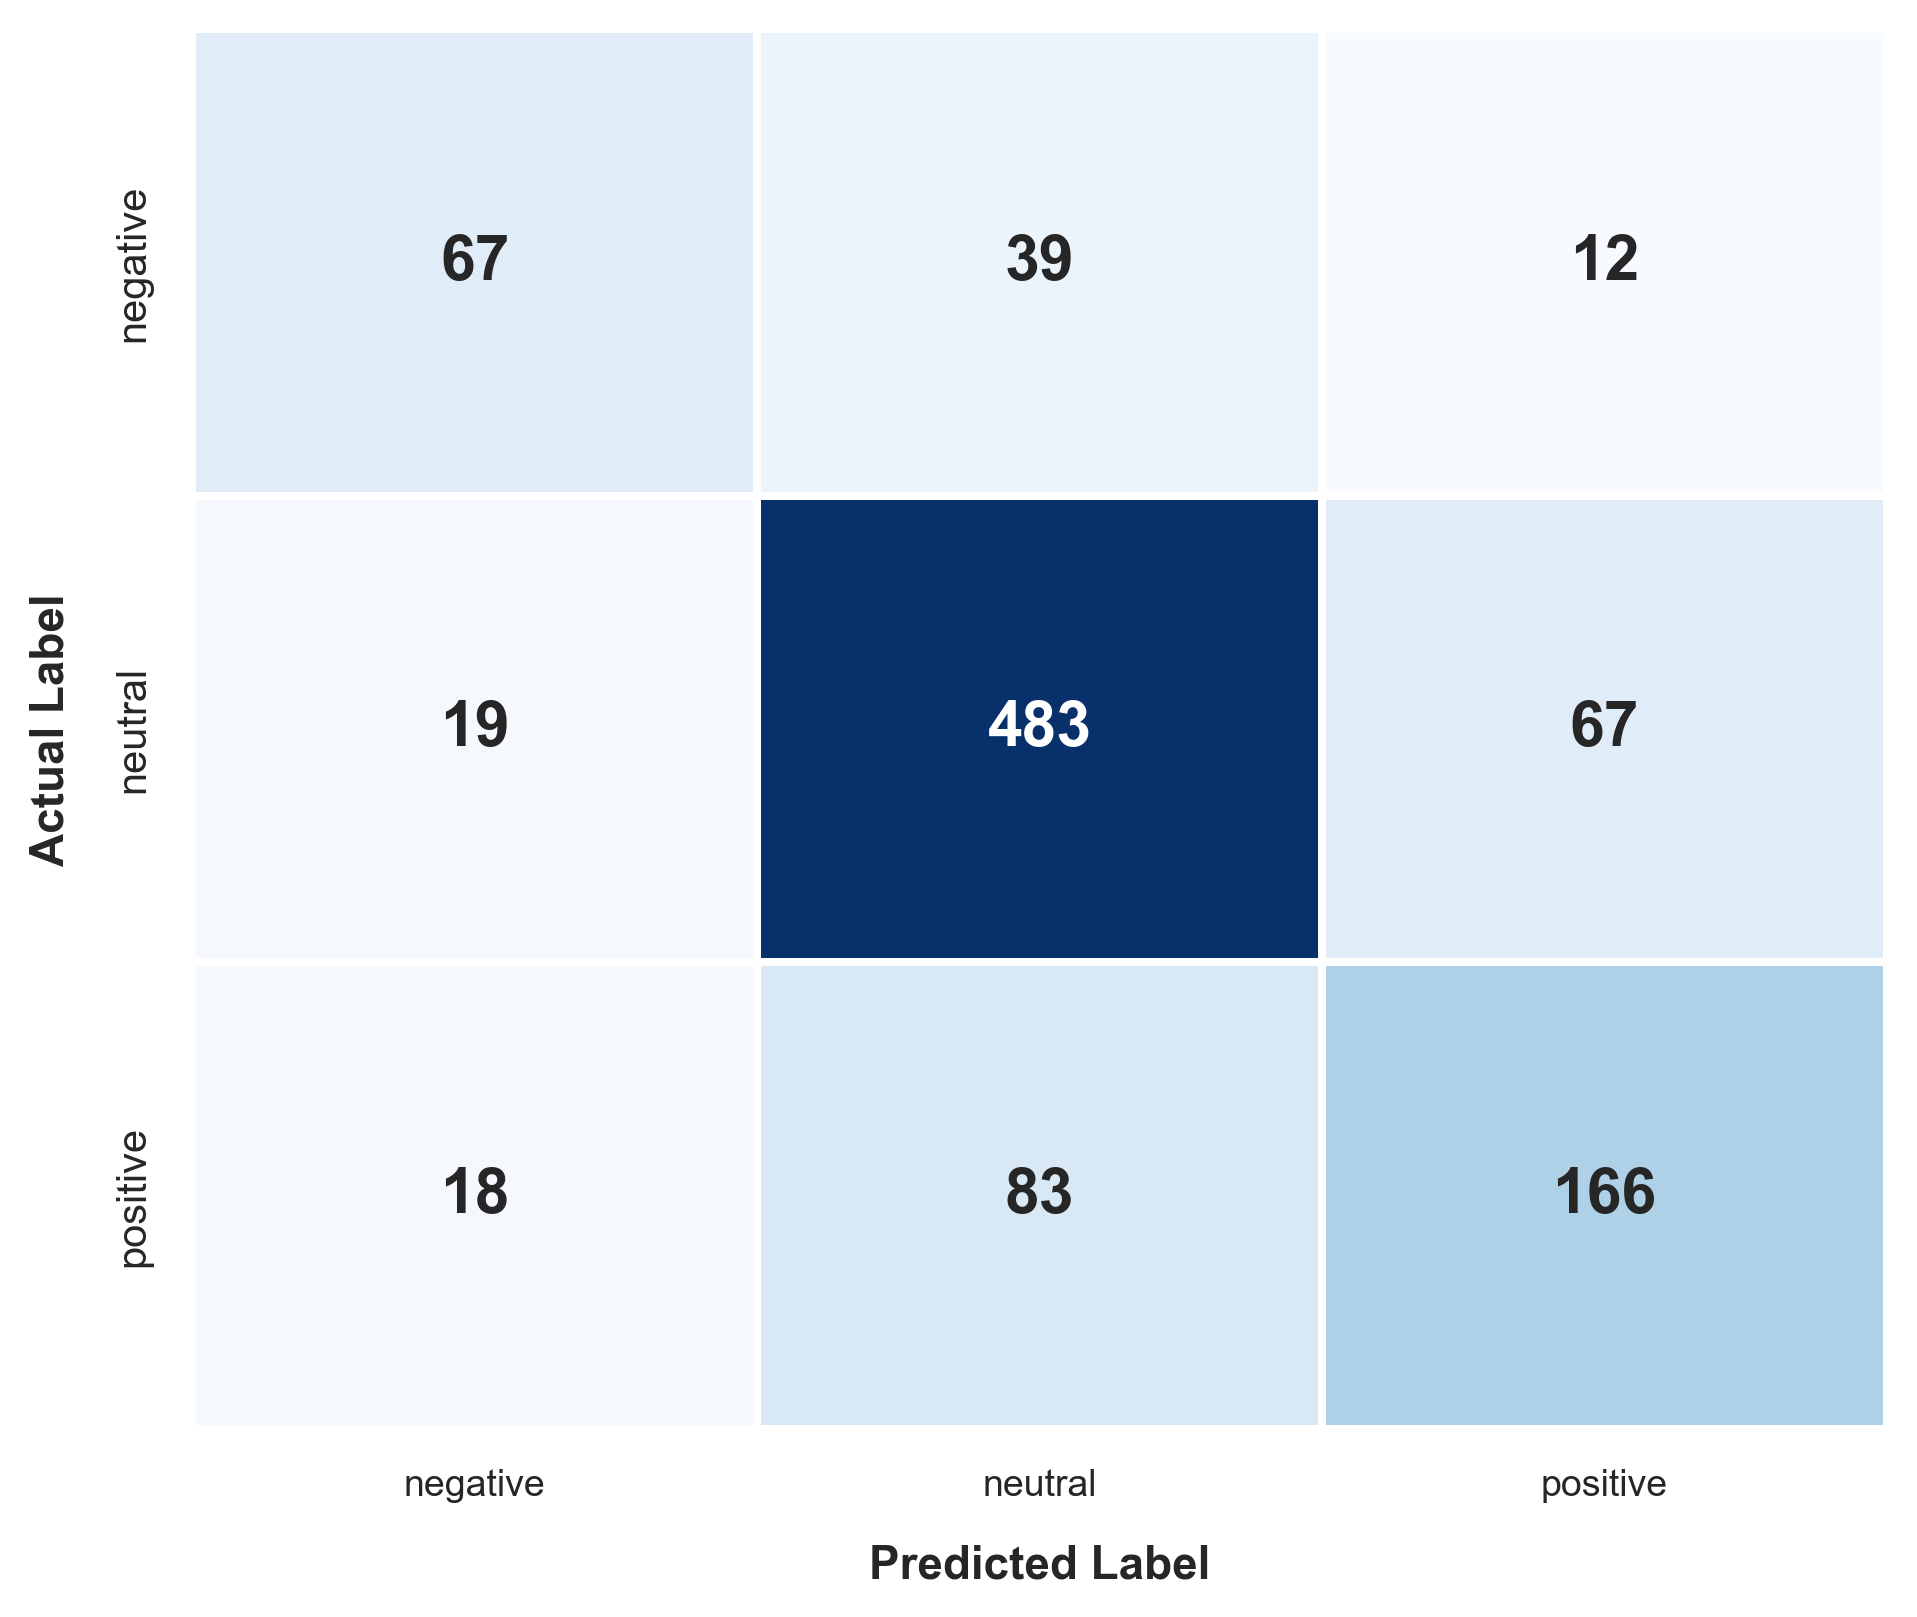
\includegraphics[width=\textwidth]{confusion_matrix_ffnn_updated.png}
        \caption*{\textbf{Best Config: \textsc{ffnn} + \textsc{tf-idf}}\\
        Strategy: ($\mathcal{S}_4$) \textbar{} $n$-Gram: (1, 2) \textbar{} TomekLink (Undersampling) \\
        Macro-$F_1$: 0.723}
        \label{fig:best_cm_ffnn}
    \end{subfigure}
    \caption{Targeted Best-Performing Performance Matrices Across Baseline Models under Optimal Preprocessing Topologies.}
    \label{fig:targeted_confusion_matrices}
\end{figure}

\section{Preprocessing Results}
\label{app:preprocessing_results}

\begin{table}[H]
    \centering
    \caption{Sample Pipeline Text Transformations and Model Predictions}
    \label{tab:pipeline_predictions_examples}
    \small
    \begin{tabularx}{\textwidth}{Xccc}
        \toprule
        \textbf{Sentence \& Masked Transformation} & \textbf{True Label} & \textbf{\textsc{ffnn} Prediction} & \textbf{\textsc{mnb} Prediction} \\
        \midrule
        ``Earnings per share \textsc{eps} amounted to EUR0 .01 .'' \newline
        \textit{``Masked: earnings share eps amount [MONEY] .''} & neutral & neutral & negative \\
        \addlinespace
        ``Europe needs 17 new large paper machines .'' \newline
        \textit{``Masked: europe need [NUMBER] new large paper machine''} & neutral & positive & neutral \\
        \addlinespace
        ``In beers , Olvi retained its market position .'' \newline
        \textit{``Masked: beer olvi retain market position''} & neutral & neutral & positive \\
        \addlinespace
        ``Gearing was 43 \% compared to 67 \% in 2004 .'' \newline
        \textit{``Masked: gearing [PERCENT] compare [PERCENT] [DATE] .''} & neutral & positive & negative \\
        \bottomrule
    \end{tabularx}
\end{table}

\section{Multiclass vs. Binary Setup Results}
\label{app:binary_metrics}

\begin{figure}[H]
    \centering
        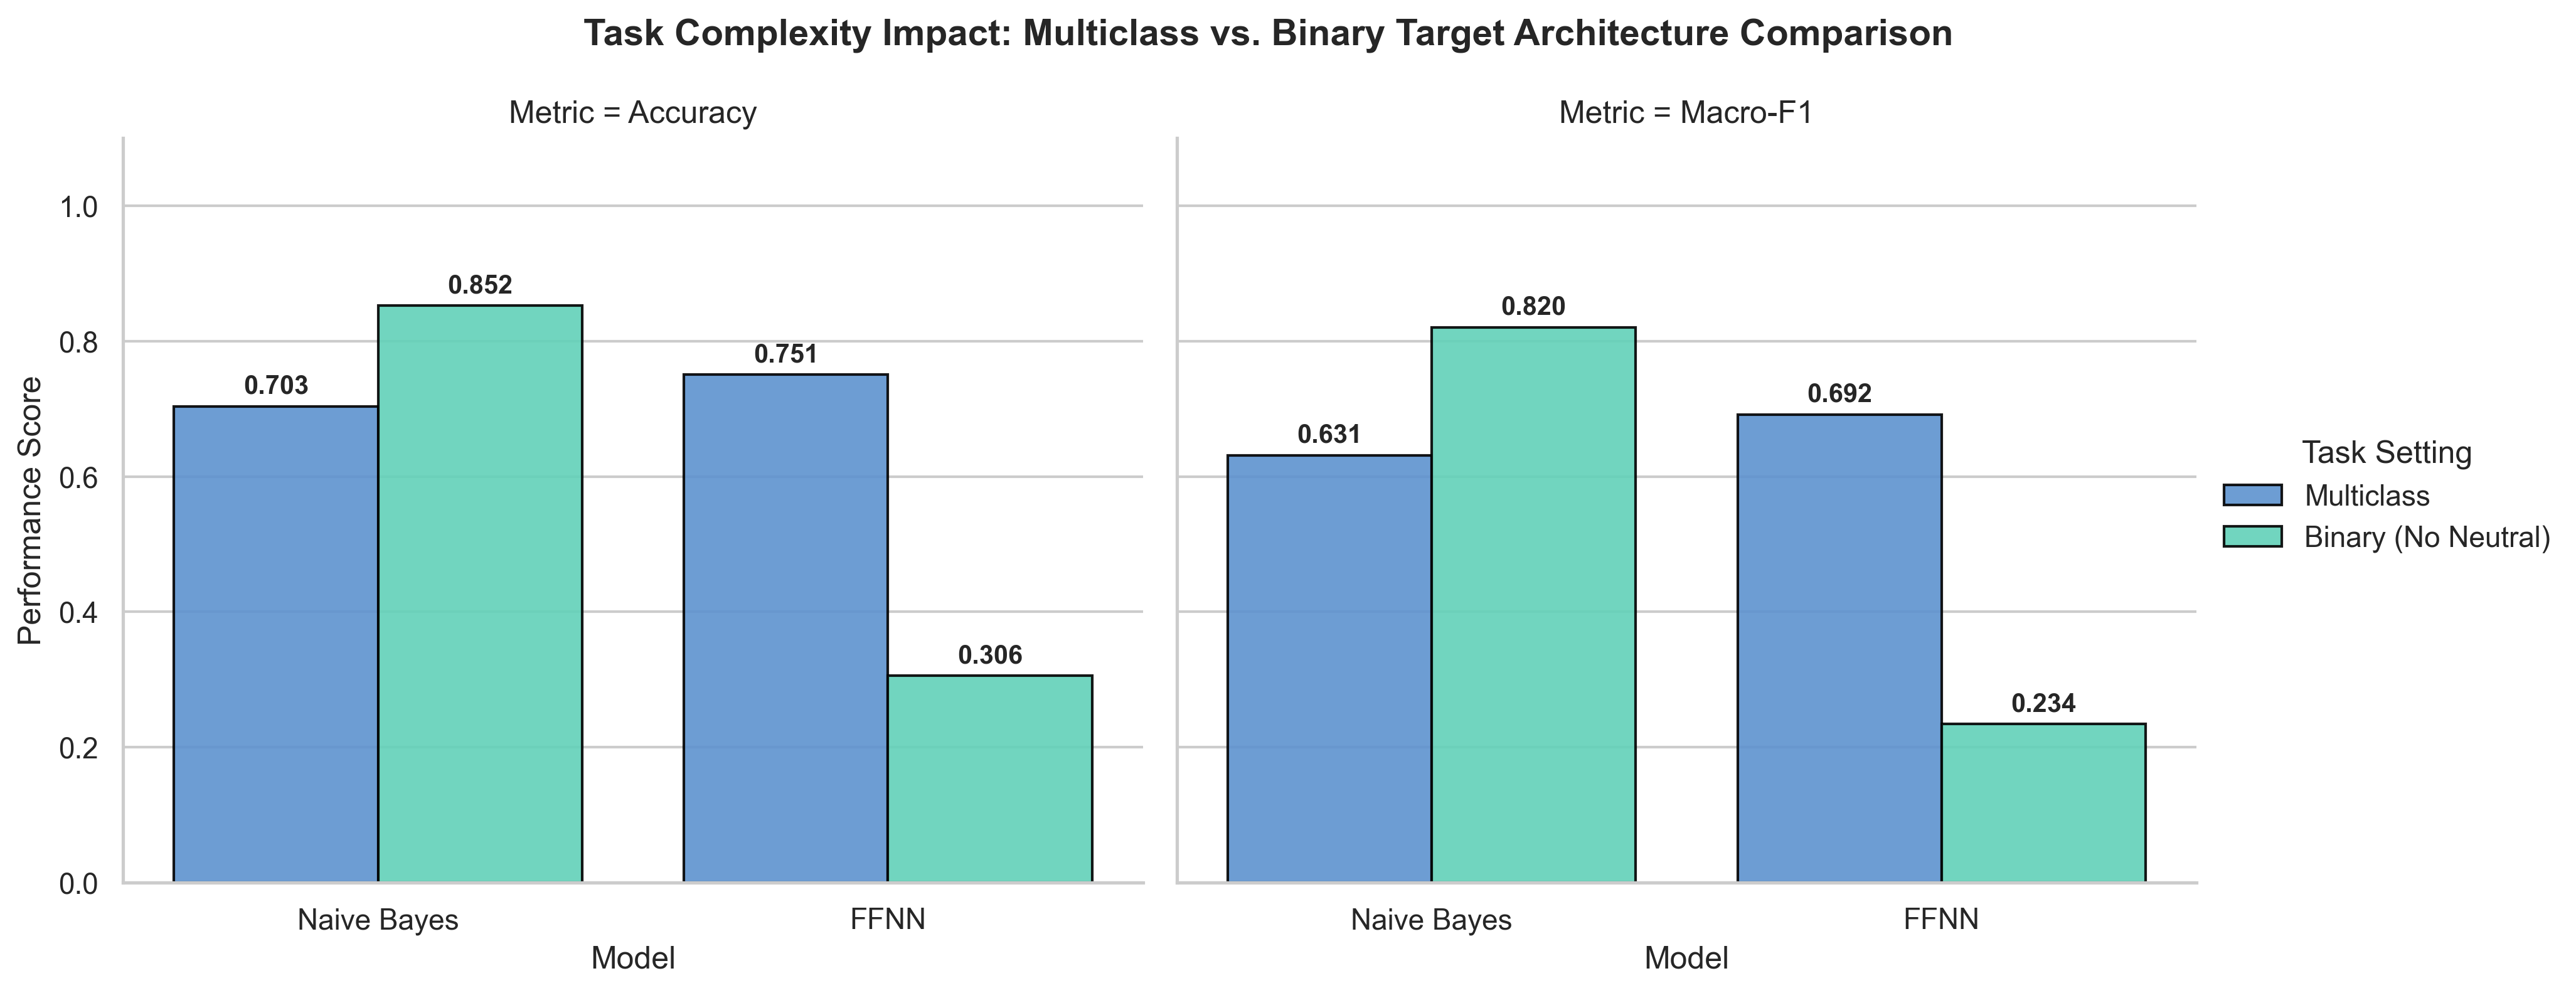
\includegraphics[width=\textwidth]{multiclass_vs_binary_comparison.png}
        \caption*{Multiclass vs. Binary Domain Metrics}
        \label{fig:mulit_binary}
\end{figure}

\end{document}
\endinput
